\documentclass{article}
\DeclareMathSizes{10}{10}{7}{7}
\usepackage{amsmath}
\usepackage{ amssymb }
\usepackage{tikz, graphicx}
\usepackage{geometry}
\usepackage[makeroom]{cancel}
\usepackage{ltablex}
\usepackage{calrsfs}
\DeclareMathAlphabet{\pazocal}{OMS}{zplm}{m}{n}
\usepackage[export]{adjustbox}
\usepackage[
backend=biber,
sorting=ynt
]{biblatex}
\addbibresource{references.bib}
\DeclareMathOperator{\sech}{sech}
\usepackage{subfig}
\usepackage[hidelinks]{hyperref}
\hypersetup{
    %colorlinks=true,
    %linkcolor=blue,
    %filecolor=magenta,      
    %urlcolor=blue,
    }
\usepackage{float}
\restylefloat{table}

\geometry{legalpaper, margin=0.7in}

\title{Noize net | WORK IN PROGRESS}
\author{Liam Watson}
\begin{document}
\maketitle
\tableofcontents
\section{Abstract}
Complete abstract at the end
\section{Introduction}
Artificial inteligence and machine learning has been a topic of much debait for many years in the theoretical space, however, in recent times advancements in computational power and theoretical models have brought these cencepts into reality. The field of machine learning is broad with many types of models such as K Nearest Neighbors, decision trees, random forests and the topic of this paper neural netowrks. These different models have midely varying structural and behavioral properties but share the same definiting principle, given some data the models have a scheme that they can use to learn how to better predict the input data whether it be for classification or time series prediction. These different models can be used to predict highly nonlinear data which before was infeasible with techniques like linear regression dominating the data analysis sphere. \\
In this paper we wish to investigate the feasibility of music generation using a class of neural network called an RNN which is specifically designed for time series data analysis.  
\section{Intorduction to Neural networks}
\label{sec:intro}
Before we procede to the more advanced recurant neural network let us begin with an abbrevated coveradge of neaural networks and the convepts underpining them. 
\subsection{Perceptrons}
\label{sec:peceptrons}
The simplest unit of a neural network is a peceptron. A perceptron is a very simple model that takes input $\{x_1, x_2, ... ,x_n\}$ along with some weights for each input $\{w_1, w_2, .., w_N\}$. The output is a binary value determined by a step function centered at some value. \cite{Nielsen} We can adjust the center point of the step function using an additional input weight, the bias $b$ which can be seen in figure 1.
\begin{figure}[H]
\caption{Peceptron showing N input variables, N weights and a bias}
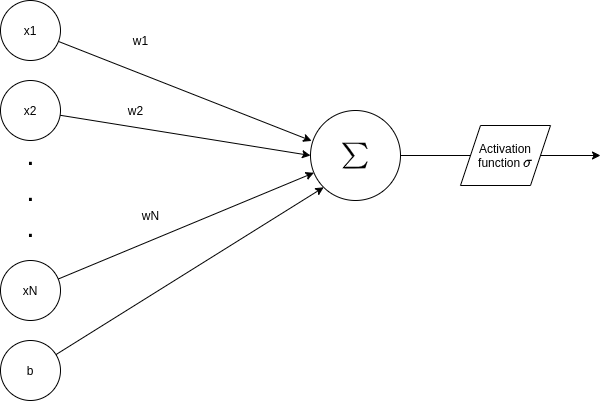
\includegraphics[scale=0.5]{peceptron.png}
\end{figure}
The output of the peceptron is calculated by point wise multiplying the weights (and bais) with the inputs, then passing the sum of the result through the step function. Mathematically this can be represented as a dot prduct of two vectors. 
\begin{align*}
\sigma \left(\begin{bmatrix}
&w_1 \\
&w_2 \\
&. \\
&. \\
&. \\
&w_n \\
&b \\
\end{bmatrix} 
\cdot 
\begin{bmatrix}
&x_1 \\
&x_2 \\
&. \\
&. \\
&. \\
&x_n \\
&1
\end{bmatrix}\right) = \sigma \left(w\cdot x\right)
\end{align*}
Given these inputs and bias we can adjust weights and bais to satisfy our desired output after summation and activation function (\ref{sec:activationfuncs}). 
More rigorously: Given some input $\{x_i\} \forall i\in \mathbb{Z^+}$ predict some $y=\sigma(W_i x_i)$ where $\sigma$ is the Heaviside step function. This model is only useful for very simple binary classification problems and has very little real world application in this form.
\subsection{Multi layer peceptrons}
\label{sec:mlp}
We only begin to see the utility when we start connecting peceptrons together in a mesh much like neurons in the brain. In figure 2 we can see a depiction of this with weights represented as line thickness (\autoref{fig:mlp}). 
\begin{figure}[H]
\caption{Image of a simple neural network archutecture with 8 inputs two hidden layers and four output neurons. Image reproduced from Ref.\cite{3blue1brown}}
\label{fig:mlp}
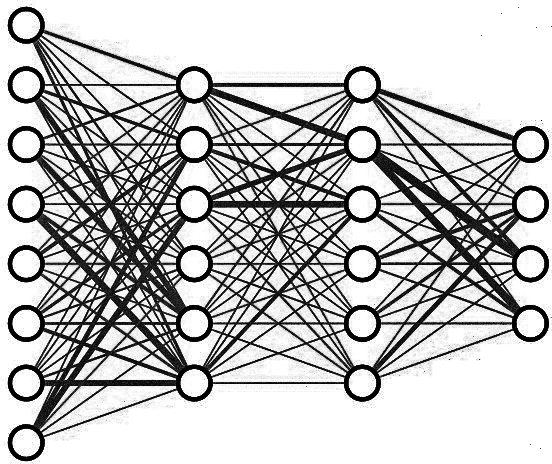
\includegraphics[scale=2]{nn.jpg}
\end{figure}
The mathematics here is similar to the single peceptron but, now the input values for any layer is determeind by the previous latyer. Mathematically this is readily represented as matrix vector multiplication. 
\begin{align*}
\sigma \left(\begin{bmatrix}
&w_{1,1} &w_{1,2} &.&.&. &w_{1,n} \\
&w_{2,1} &w_{2,2} &.&.&. &w_{2,n}  \\
&.&.&.&.&.&. \\
&. &.&.&.&.&.\\
&. &.&.&.&.&.\\
&w_{n,1} &w_{n,2} &.&.&. &w_{n,n}  \\
\end{bmatrix} 
\begin{bmatrix}
&x_1 \\
&x_2 \\
&. \\
&. \\
&. \\
&x_n \\
\end{bmatrix}
+
\begin{bmatrix}
&b_1 \\
&b_2 \\
&. \\
&. \\
&. \\
&b_n \\
\end{bmatrix}
\right) = \sigma \left(\textbf{W} \vec{x} + \vec{b}\right)
\end{align*}
Where the activation function is applied to each of the resulting vector elements. 
\subsection{Activation functions}
\label{sec:activationfuncs}
Now we will discuss, much like with a biological neuron, how will a neuron decide to acivate or not. A binary step function is very limiting in terms of application to the real world, a continuous output would be far more useful for classicication probabilities or in our case of this work, music generation. There are many functions that are used in the literature but here we give give a quick overview of the most common functions and their uses. The purpose of an activation function is to format the output of a peceptron, we begin with the most elementary of these functions (excluding the identity function defined as $f(x) = x$. 
\begin{enumerate}
\item The binary step function \\
Definition:
\begin{align*}
f(x) = 
\begin{cases}
 1 & \text{if } x > 0 \\
 0 & \text{if } x \leq 0 \\
\end{cases}
\end{align*}
\begin{figure}[H]
\centering
\caption{A plot of the Heaviside step function}
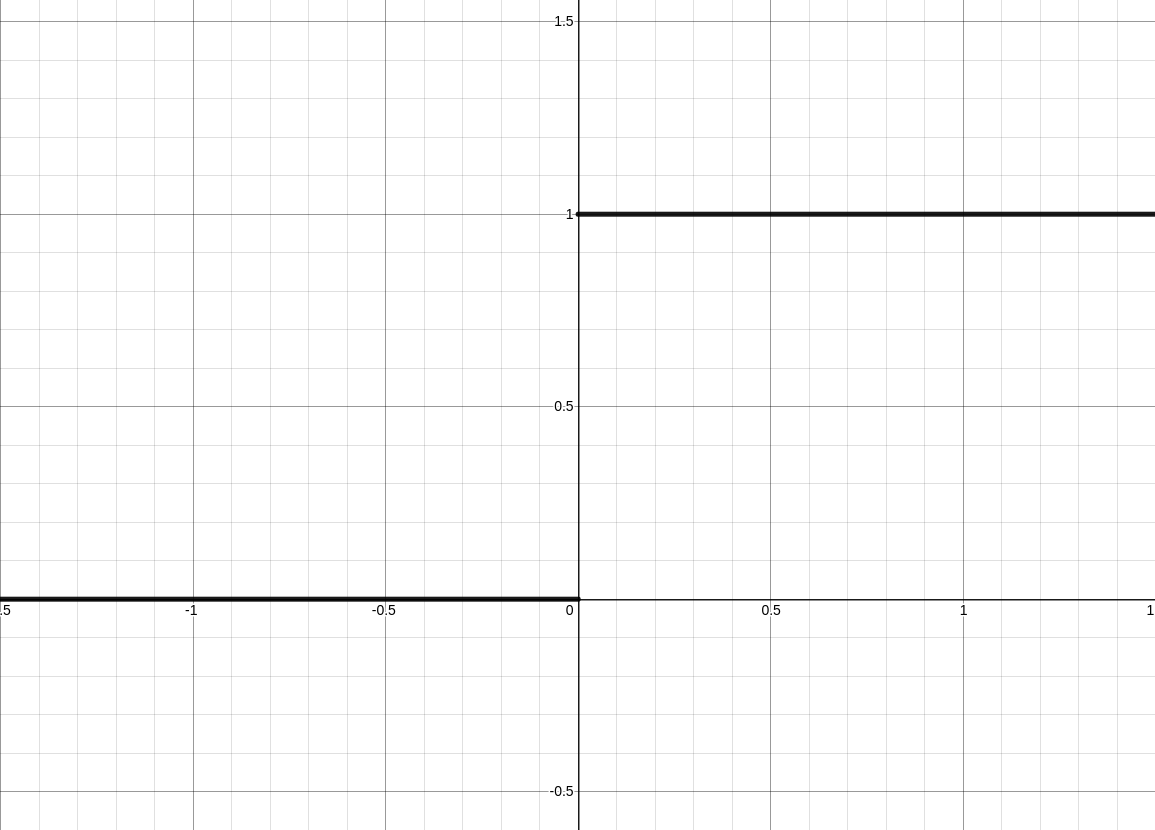
\includegraphics[scale=0.2]{heaviside.png}
\end{figure}
The binary step function is primarly used for true, falue classification where the result is not a probability but a certanty. Beyond this this activation function has limited use in modern neural networks, hoever it should be noted that it is very computationally efficient. 
\item Rectified Linear Unit(ReLU)\\
Definition: 
\begin{align*}
f(x) =
\begin{cases}
 0 & \text{if } x \leq 0 \\
 x & \text{if } x > 0 \\
\end{cases}
\end{align*}
\begin{figure}[H]
\centering
\caption{A plot of the ReLu function}
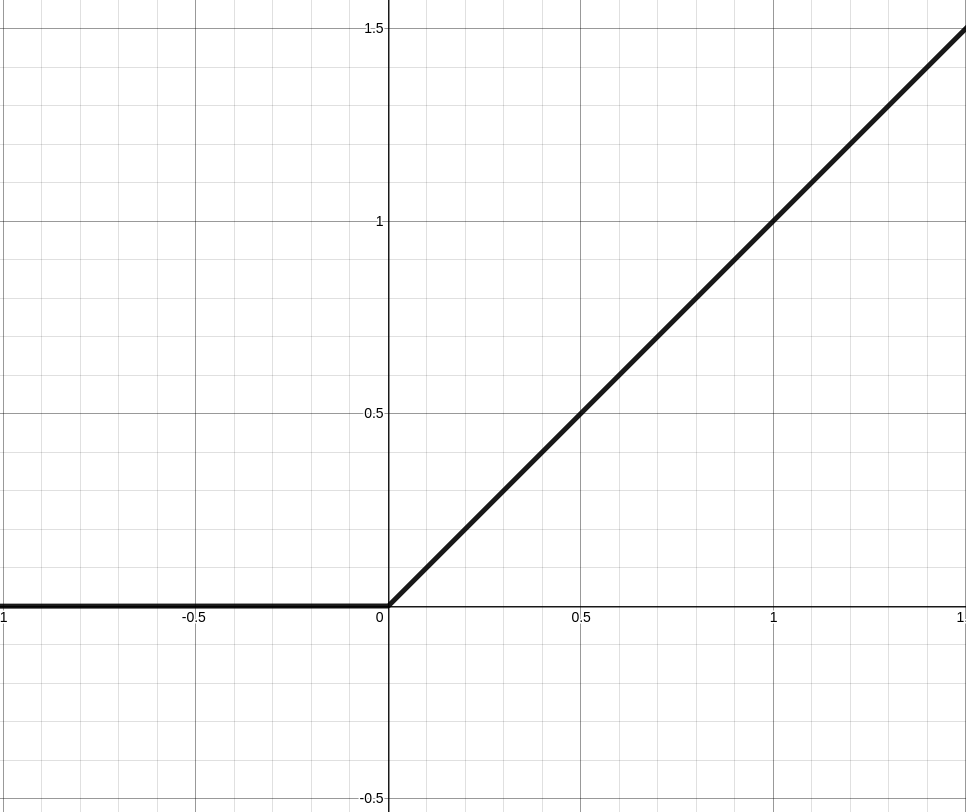
\includegraphics[scale=0.2]{relu.png}
\end{figure}
The ReLU Function finds much use dispite its simplicity mostly due to its computational efficiency when compared to the more complex activation functions. ReLU reduces the input domain to only non-negative numbers which can be useful in cases where one wishes to disregard such values. 
\item Sigmoid \\
Definition: 
\begin{align*}
&f(x) = \frac{1}{1 + e^{-x}}
\end{align*}
\begin{figure}[H]
\centering
\caption{A plot of the sigmoid function}
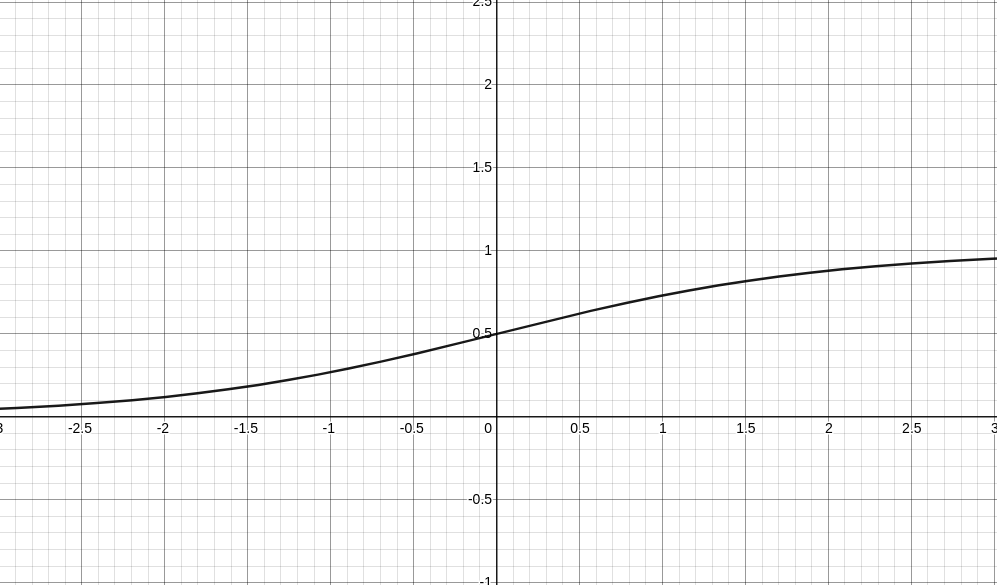
\includegraphics[scale=0.2]{sigmoid.png}
\end{figure}
\item Hyperbolic Tangent\\
Definition:
\begin{align*}
f(x) = \frac{e^x - e^{-x}}{e^x + e^{-x}}
\end{align*}
\begin{figure}[H]
\centering
\caption{A plot of the $\tanh$ function}
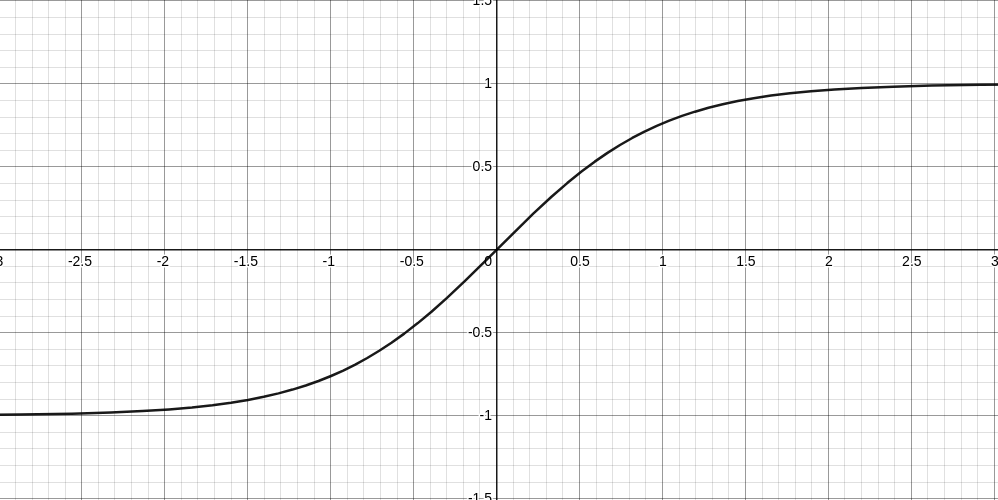
\includegraphics[scale=0.2]{tanh.png}
\end{figure}
\end{enumerate}

\subsection{Feed forward}
\label{sec:forward}
Now we have covered how to calculate the activations of each neuron in the netowrk, we can now begin using the output. The output of the network is obtained during the feed forward stage of a network. The network will recieve input's at the input neurons and propagate through all the network layers calculating sum's and activations until the algorithm reaches the output layer. The activations at the output layer are considered the network prediction. One can see why the phase is called feed forward, as the network propagates activations "left to right", forward through the network. 
\subsection{Error functions (Loss functions)}
\label{sec:error}
Once we have output from the model, we need a metric for the error between the output prediction and ground truth, an error function. There are many error functions that appear in the litterature, however, their use is often highly application dependent. In the case of music generation we are dealing with simple two dimensional time series data and as such the relevant error functions are elementary:
\begin{enumerate}
\item Mean Square Error (MSE)\\
This error function finds the averadge square difference between the predicted value and ground truth, defined as
\begin{align*}
MSE = \frac{\sum_{i=0}^N (y_i - y_i^\prime)^2}{N}
\end{align*}
Where $N$ is the number of output values, $y_i$ is the ground truth value and $y_i^\prime$ is the predicted value. \\
This loss function is favorable because of it's simplicity and computational efficiency. One should note that MSE can "amplify" large errors and squah small errors due to the square and notice that the direction of the error is also ignored.  
\item Mean absolute error \\
If one would not like to square the error in order to better capture small errors one can use the MAE function which shares many similar properties with the MSE function but more accurately depicts the difference between a prediction and the ground truth. 
\begin{align*}
MAE = \frac{\sum_{i=0}^N |y_i - y_i^\prime|}{N}
\end{align*}
\item Mean Bias error \\
If the appliction requires a signed error function the MBE error function could be applicable. However, one should note that possitive and negative values may cancel each other out leading to unpredicatble results in practice. 
\begin{align*}
MBE = \frac{\sum_{i=0}^N (y_i - y_i^\prime)}{N}
\end{align*}
\end{enumerate}
It should be noted that more complex loss functions are used for categorical data such as cross entropy loss or hinge Loss.

\subsection{Gradient decent}
\label{sec:gradientDecent}
Now we need a method to update the peceptron weights given some value for the error between some prediction and ground truth, for this we use gradient decent. There are many adaptions of gardient descent that aim to optimize its computational performance or over come some issue with converging to a poorly optimised solution such as fast gradient methods or momentum adapted gradient descent methods. \\
The aim of gradient descent is to itteratively optimize the peceptron weights in order to converge on a minimum (likely a local minimum) by taking steps in the direction of steepest descent, after many itterations we will find that the networks weights are well optimised for some goal. However we may find that a local minimum is not sufficient for our purposes and as such may need to employ some hyperparameter tuning such as changing the the step size we take or adding momentum in the hopes that we converge to a more optimal solution.
\begin{figure}[H]
\centering
\caption{A plot of $f(x,y) = \sin(x) + \sin(y)$ with a path showing gradient decent steps}
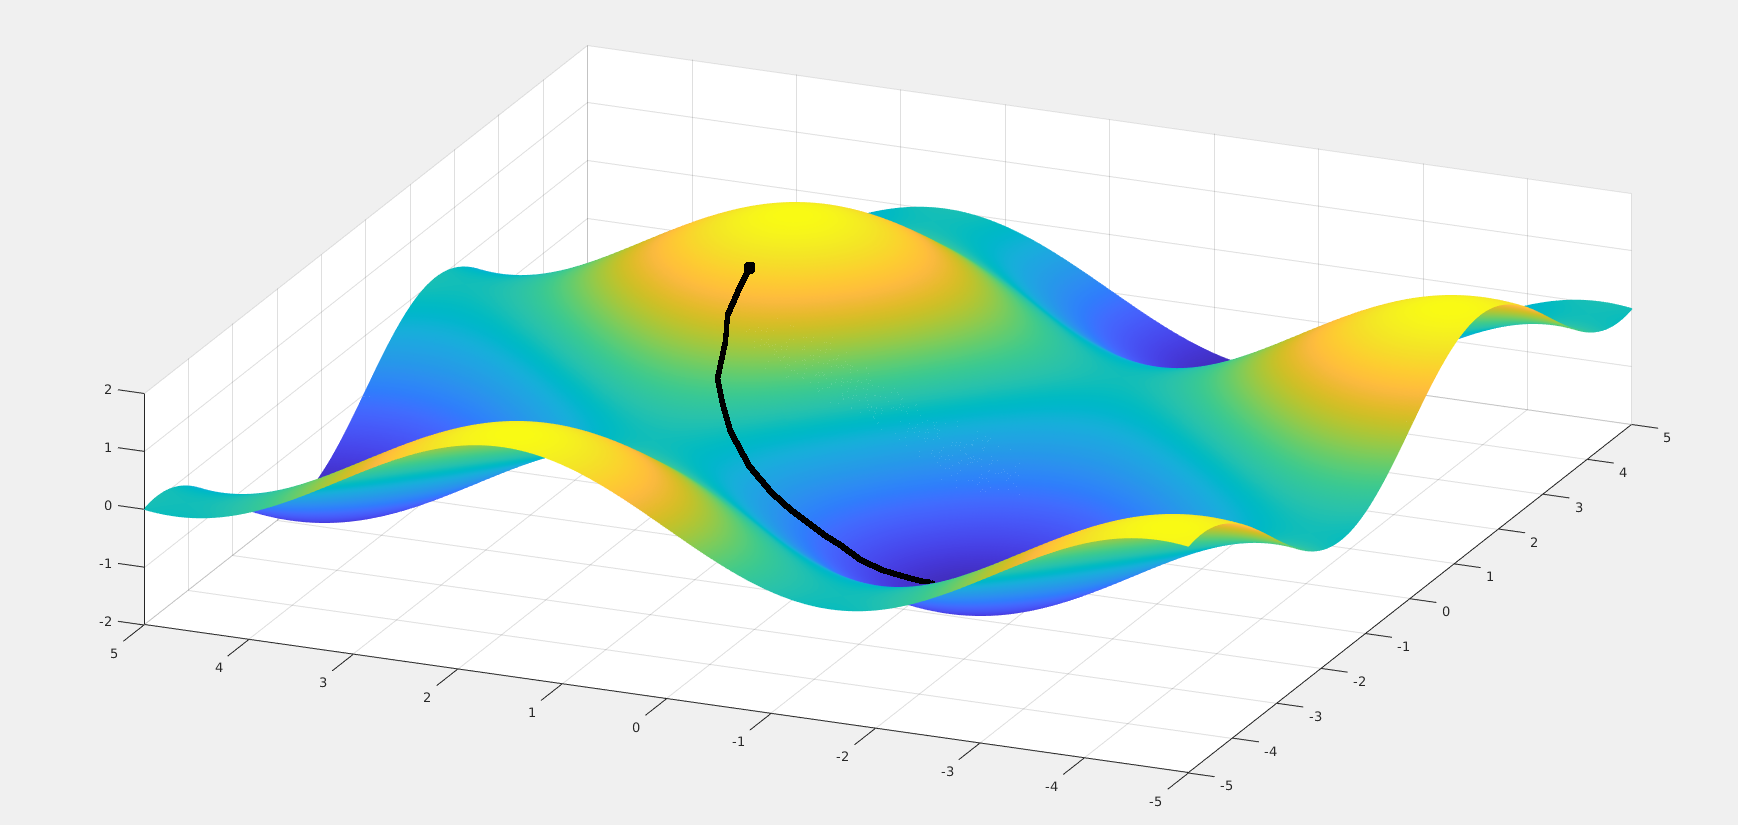
\includegraphics[scale=0.2]{mesh.png}
\end{figure}
Mathematically gradient descent is a simple optimization problem. First we must define cost. The cost is defined by some error function as discussed above where in the context of a neural network we sum the "difference"(absolute, sequared or standard) between each of the output neurons and the ground truth value, then divide by the number of output neurons. So if we have some function that calculates the cost (a so called cost function $C$) we can calculate the gradient $\nabla C$ and take a step in the opposite direction $-\nabla C$ as we wish to find the minimum of the cost function. 
\subsection{Back propigation}
\label{sec:back}
Back propigation is the learning step for a model. Once we have completed the feed forward step and calculated the error we need to travel back through the network and adjust the weights and biases in order to optimize the model. In order to update the weights and bais values we need to know by how much.  
NB: We need to add the maths here 

\section{Intorduction to Recurrant Neural Networks}
\label{sec:intoRNNs}
When using neural networks for time series data prediction, some semblance of memory is required for sucsessive predictions. Unfortunately standard multi-layer peceptron and convolutional neural networks tend to lose this information quickly as they train due to the vanashing gradient problem. RNNs seek to resolve this by constructing hand crafted compositions of so called "gates" that can encorperate prior information for sucsessive predictions. 

\subsection{RNN concepts}
\label{sec:RNNS}
NB refactor this section
RNNs are designed specifically to learn from sequences of data by passing the hidden state from one step in the sequence to the next step in the sequence, combined with the input. This gives RNNs the ability to predict sequences of values using knowledge of past state as well as current state. 
\begin{figure}[H]
\caption{RNN basic architecture}
\label{fig:RNN}
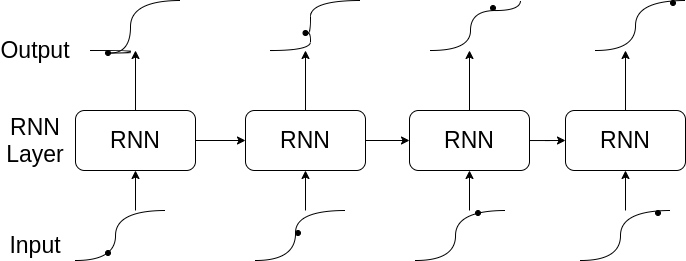
\includegraphics[scale=0.5]{RNN.png}
\end{figure}
The more rigorous definition of an LSTM is as follows:
\begin{align*}
h_t = \tanh\left( W_{ih}x_t + b_{ih} + W_{hh}h_{t-1} + b_{hh}  \right)
\end{align*}
With $h_t$ being the hidden state at some time $t$ that is passed forward to the next recurrant unit at $t+1$. Then $W_{jj}$ is some weight vector, $x_t$ the input vector and $b_{jj}$ some bias vector. In this paper we will exlusivly use $\tanh$ as the nonlinearity, however, it is common for the $ReLU$ function to be used. \\
RNNs performs well on sequential data, however, in large time scales the model is likely to suffer from poor long term memory due to repeated gradients deminishing exponentially in time, the so called vanashing gradients problem. An additional contributor to the standard RNNs poor long term memory is that after each RNN cell we pass data through an activation function, which over many repeated transformations can result in loss of the meaning of the original information in the data. 
\subsection{LSTM}
\label{sec:LSTM}
Long short-term memory (LSTM) is an extension to the idea of an RNN in that sequential data can be predicted by passing the hidden state of LSTM cells forward in time, however, a more sophisticated design of each unit in an attempt to mitigate information loss due to repeated data transformations and the vanashing gradients problem. The overall architecture of the LSTM cell is displayed bellow and in the following sub sections I will break down what each piece of the cell does and why it is included. 
\begin{figure}[H]
\caption{LSTM cell \cite{LSTM}}
\label{fig:RNN}
\includegraphics[scale=0.4]{LSTM_cell.png}
\end{figure}
The above figure is complex, however, we can combine the operations into four distinct functional components ("Gates") namely: Learn, forget, remember, and use gates. Each of these four gates has a specific intended function, however, it is pertinent to note that with statistical models there is little rigorous reasoning to why their structure. By combining the follwing gates (or adding new ones) in novel ways one can form their own cell with desired properties. Another cell commonly reffered to in the litterature is the Gated Recurrant Unit (GRU) which has a lower computational cost than the LSTM as it only uses two gates, namely the update and reset gates.\\
Note: The cell state is sometimes reffered to as the long term memory and the hidden state the short term memory.
\subsubsection{The Learn Gate (Input gate)} 
The Learn gate determines which information from the hidden state and input should enter the cell state. This is accomplished by passing the previous hidden state $h_{t-1}$ and input $x_t$ through a sigmoid (producing $i_t$) and $\tanh$ activation ($g_t$) functions and combining the results in point wise multiplication.
\subsubsection{The Forget Gate} 
The forget gate $f_t$ is included to determine which information can be ignored or emphasised. The forget gate takes in some input $x_t$ and some previous hidden state $h_{t-1}$ which are passed through a sigmoid activation function. The result of the sigmoid function is between 0 and 1 with 0 implying the data is irrelevant and a 1 indicating the data is highly valuable. The output of the forget gate is then used in the cell state operation to find $c_t$.
\subsubsection{The Remember Gate (Cell State)} 
The remeber gate is, in essence a combination of the previous cell state $c_{t-1}$ with the infomration produced by the forget gate (using point wise multiplication) and then the input gate $g_t i_t$ using point wise addition to produce a new cell state $c_t$. This scheme is an attempt to calculate the most valuable new cell state.
\subsubsection{The Use Gate (The output gate) } 
The use gate is used to produce the new hidden state $h_t$ using the most relevant information from the previous hidden state $h_{t-1}$, input $x_t$ and cell state $c_t$. First we process the previous hidden state and input by passing them through a sigmoid activation function, the result being some $o_t$. Then we can calculate the new hidden state $h_t$ by point wise multiplying $o_t$ and the result when passing the cell state through a $\tanh$ activation function.


With the macro definition of the LSTM cell we can print the rigorous mathematical definition which is as follows \cite{LSTM}\cite{sak_senior_beaufays_2014}:
\begin{align*}
&i_t = \sigma\left(W_{ii}x_t + b_{ii} + W_{hi}h_{t-1} + b_{hi} \right) \\
&f_t = \sigma\left(W_{if}x_t + b_{if} + W_{hf}h_{t-1} + b_{hf} \right) \\
&g_t = \tanh\left(W_{ig}x_t + b_{ig} + W_{hg}h_{t-1} + b_{hg} \right) \\
&o_t = \sigma\left(W_{io}x_t + b_{io} + W_{ho}h_{t-1} + b_{ho} \right) \\
&c_t = f_t \odot c_{t-1} + i_t \odot g_t \\
&h_t = o_t \odot \tanh(c_t)
\end{align*}
Where $\sigma$ is the sigmoid function, $\odot$ is the Hadamard product (element wise product), $c_t$ is the cell state at some time, $h_t$ is the hidden state at some time, $i_t$ is the input gate, $f_t$ is the output gate, $g_t$ the cell gate, $0_t$ is the output gate and $x_t$ is the input data at some time. $W_{jj}$ are the input weights and $b_{jj}$ is the input bias. 
\section{Noize net}
\label{sec:nn}
\subsection{Data and preprocessing}
The data used for training, validation and prediction is the free music archive which includes songs labelled with many usefull charatersistics, particularly interesting to us is genre.  \cite{fma_dataset}
\cite{fma_challenge}
\subsubsection{Digital Music}
In this section I will briefly discuss why RNN's are a favourable model of choice for digital music generation. \\
Sound is fundamentally a time series phenomenon, being the pressure of a medium in space. When we sample sound using a microphone, we record the voltage changes in an inductor that is actuated by the changing pressure of the air. These voltage values can then be scaled by some scaling function determined by a manufacturers testing. The output file can then be viewed as many amplitude values in some complex wave traveling in time. There is some complexity with compression formats such as the mp3 standard which are taken care of by the librosa library. \cite{isoMP3}
\subsubsection{An introduction to digital sound representations}
Now that it is clear how digital audio is stored, in this section I will briefly discuss the different representations of digital audio and why we use them. \\
Firstly, follwoing from the above section on digital music we can see the sample view which is an intuitive plot showing the sample amplitude against time. These plots are useful to us for checking the quality of the data produced by our model as we can clearly see if there is any irractic non-music like data. This view, however, gives us little indication of the qualitative aspects of the music produced by a model. 
\begin{figure}[H]
\caption{Example spectrogram taken \cite{mcfee2015librosa}}
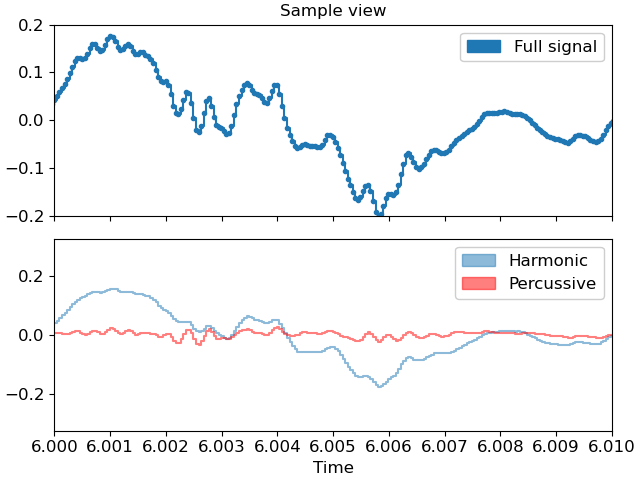
\includegraphics[scale=0.5]{librosa-display-waveshow-1_01.png}
\end{figure}
The next representation to be aware of is the envelope view which shows the amplitudes as did the sample view, however, this view makes reading off qualitative aspects of the music simple. The envelope is often used by muscisions, who will often use the ASDR interpretation of each progression in the graph. \cite{vail_2013}
\begin{figure}[H]
\caption{Example spectrogram taken \cite{mcfee2015librosa}}
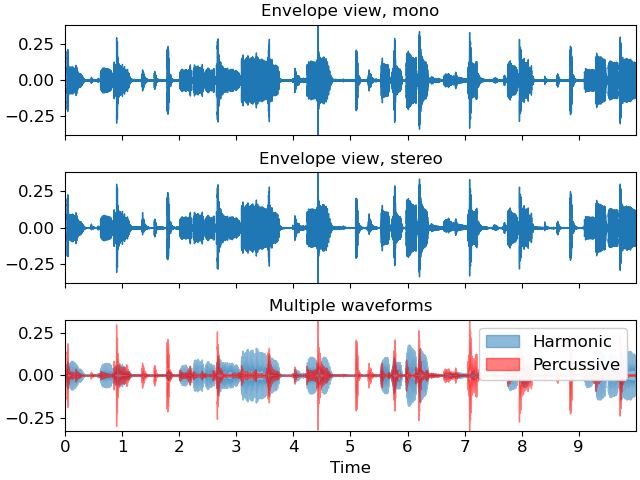
\includegraphics[scale=0.5]{librosa-display-waveshow-1_00.png}
\end{figure}
The last audio representation we will use in this paper is the spectogram which is a heat map with frequency (logarithmic or linear) on the vertical axis, time on the horizontal axis and temperature representing volume. The spectogram is often used in scientific audio applications as it gives us a clear plot showing the distripution of frequency and volume which we can use to describe both qualitative and quantative aspects of the data produced by a model. 
\begin{figure}[H]
\caption{Example spectrogram taken \cite{mcfee2015librosa}}
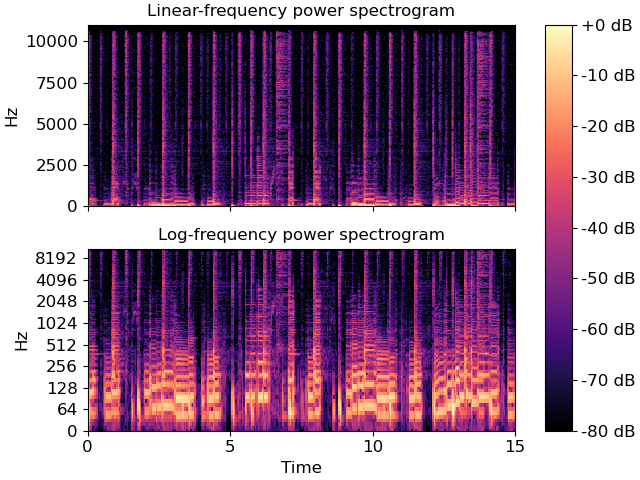
\includegraphics[scale=0.5]{librosa-display-specshow-1.png}
\end{figure}
\label{sec:data}

\subsubsection{Additional data representation}
Now that it is clear how digital music is represented we can discuss an additional representation of the data. One may question why we seek a different representation, which is a fair question. The musical data in its current format although periodic, is highly nonlinear as decisions made by the artist are somewhat arbitrary without much underlying variable dependence. This is especially true in modern music where triditional notes, tempo and other musical norms are ignored, favoring intuative qualitative enjoyment of a song. This philosophy to music design results in the underlying sound data being highly eratic and lonlinear which neccesitates a more complex model to capture the highly nonlinear behavior. In the two figures bellow one can see the differences between a classical and a modern instrumental song.
\begin{figure}[H]
\caption{Envelope plots demonstrating classical vs Instrumental music nonlinearity}
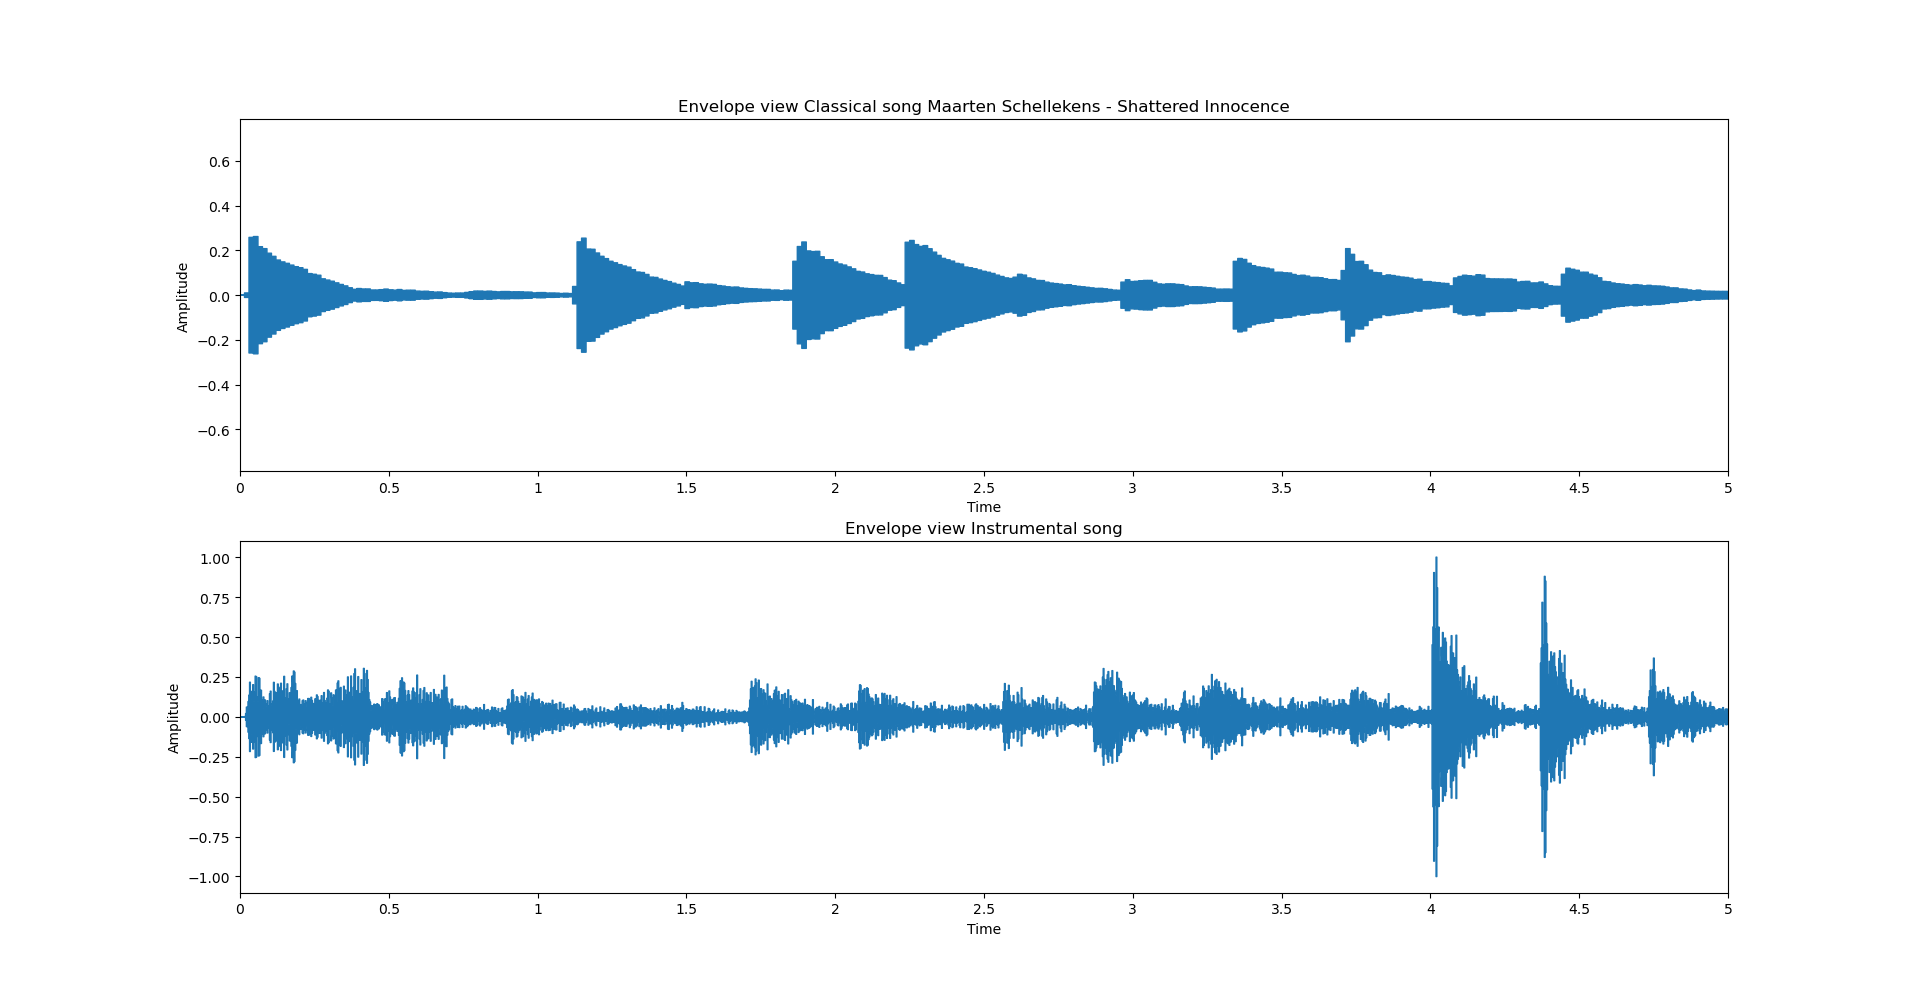
\includegraphics[scale=0.35]{Classical_vs_Instrumental.png}
\end{figure}
In order to extract more useful information from the data we can transform some input song using a discreet fourier transform (namely the fast fourier transform scheme (FFT)). A fourier tranform of the amplitude domain data results into frequency domain data. This new representation should better yeild teporal frequency information such as chords or notes to the model. Bellow we can see a modern instrumental song in amplitude and frequency domains. 
\begin{figure}[H]
\caption{Envelope plots demonstrating classical vs Instrumental music nonlinearity via FFT}
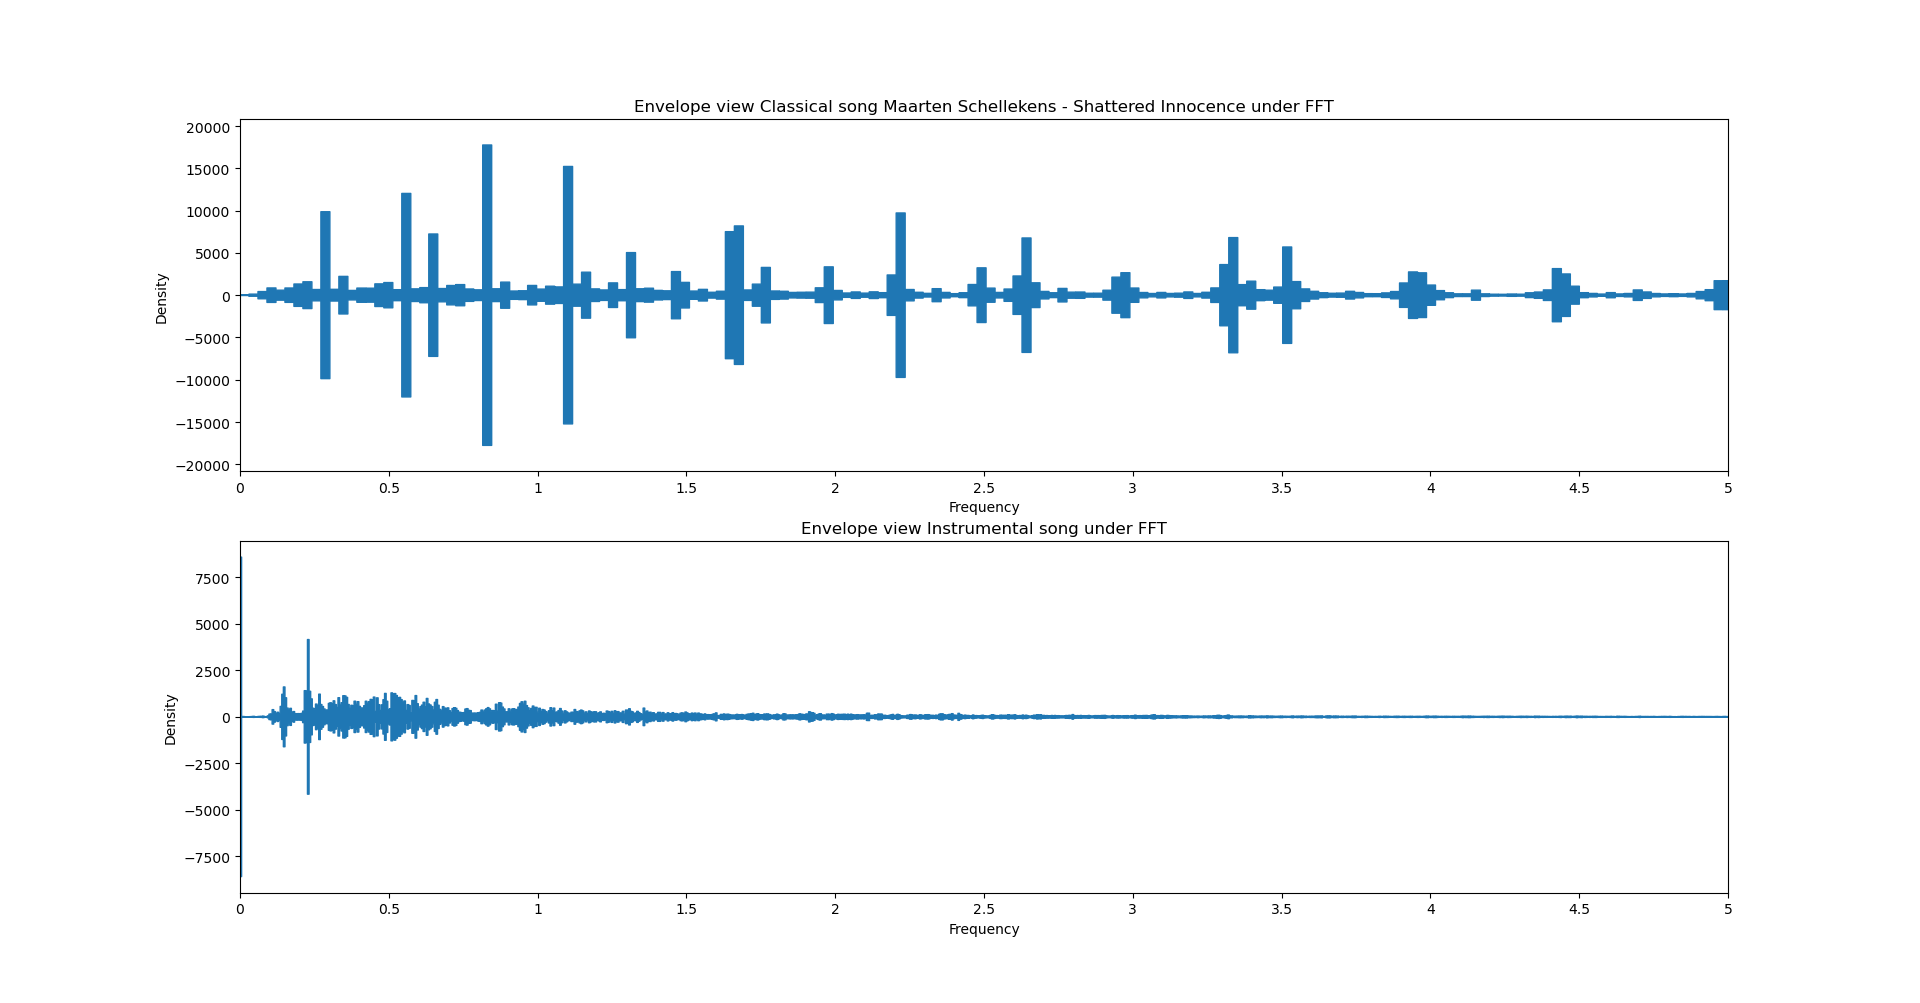
\includegraphics[scale=0.35]{Classical_vs_InstrumentalFFT.png}
\end{figure}
\subsubsection{Data used for generation seed}
In order to generate novel music we need to give the model some initial data to being prediction refered to as the seed. In this work we will be using three different seeds namely: An unseen instumental song, random noise and perlin noise.
\begin{enumerate}
\item The instrumental song used as a seed is completely unseen by the model. That is to say the seed is not in the training data. We expect this seed to produce the highest quality results as it is the most similar to the data used in training.
\item The random noize is generated from python's pseudo random number generator and qualitatively sounds like static noise. The reason for the inclusion of this seed is to experiment with how well the model retains an understanding of music when given a completely random input.
\item The perlin noise is included as an interesting sub set of the random seed as perlin noise contains qualitatively reconisable sounds which may aid the generation of novel music. How pelin noise works is beyond the scope of this paper but for the readers convenience \href{https://adrianb.io/2014/08/09/perlinnoise.html}{here} is an explantion.
\end{enumerate}

\subsubsection{Data scaling}
Scaling the input data is an important step in the preprocessing for many reasons. Here is a list of the reasons to normalise data:
\begin{enumerate}
\item Prevent neuron saturation
\item Enphasize imporant relations in the data
\item Smoothing input data 
\item Aiding stable convergence of gradients
\item Prevents likelyhood of overfitting
\end{enumerate}
There are many different data scaling techniques which may perform differently on different data sets. A list of the most common teqniques:
\begin{enumerate}
\item Linear Scaling
\item Clipping 
\item Log Scaling
\item Z-score
\end{enumerate}
In this paper work we will use Z-scaling as data scaling includes negative values and performs well under testing. It should be noted, however, that as with most choices here the choice is heurist based and there may be a better choice that performs better under certain conditions. The implimentation makes use of scikit learn's standard scaler\cite{scikit-learn}.
\subsection{Architecture of NoiseNet}
\label{sec:arch}
Due to music having natural time dependence and periodicity it is wise to develop some recurrant architecture. In this paper we will use a standard RNN as well as an LSTM. Both these models should produce similar predictive behavior with the LSTM expected to exhibit better long term memory characteristics than the standard RNN. \\
The architecture of the model will consist of several layers: the input layer which typically would include some kind of normalisation or embedding,  RNN  layers, a fully connected layer to trlanslate the RNN layers output and an output layer. These layers are depicted in the figure bellow:
\begin{figure}[H]
\caption{Example of NoizeNet architecure demonstrating how music prediction will work}
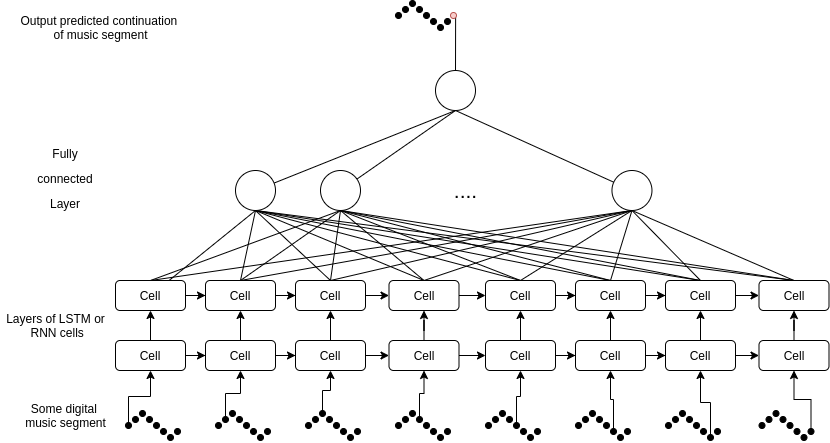
\includegraphics[scale=0.5]{NoizeNetArch.png}
\end{figure}
\subsection{Implimentation}
\label{sec:impl}
The implimentation for this paper was completed in python with the follwoing framewroks and libraries:
\begin{enumerate}
\item PyTorch library for Neural Networks \cite{NEURIPS2019_9015}
\item Librosa for audio I/O \cite{mcfee2015librosa} 
\item Matplot lib \cite{Hunter:2007} and Librosa display \cite{mcfee2015librosa} for graphics rendering
\item Scikit learn \cite{scikit-learn}, pandas \cite{reback2020pandas} \cite{mckinney-proc-scipy-2010}, librosa \cite{mcfee2015librosa} and numpy \cite{harris2020array} for data processing \cite{fma_dataset}\cite{fma_challenge}
\end{enumerate}
Please see the code repositorty \href{https://github.com/Liam-Watson/NoizeNet}{here}. Included in the repository are the figures used in this paper, an implimentation of the RNN and LSTM models, a few faved models with varying hyperparameters that will be analysed bellow along with the seeds used to generate them and the predicted sound file. 

One should note that the implimentation yields many hyperparameters that can be used to optimise the results produced by a model or the model performance. This is important to this investigation as audio data is very large. The sample rate used in this implimentation in 22050Hz, so for a 30 second section of music we find $6.615\cdot 10^{5}$. The large size of data implies, necessarily a very large model, many training/prediction steps and high memory usage. \\
Due to this many hyperparameters had to be tuned for compuational performance rather than model optimization. \\
The high memory requirement is also of note as one has to ensure that any unused memory is cleaned up frequently by the garbage collector. In python this is a relatively trivial procedure but is of note. 

\subsubsection{Hyper-parameters}
There are many factors that can effect a neural network model's performance, the factors that one can control are reffered to as hyper-parameters. In the table bellow I have include some of the hyperparamets that may influence both the RNN's ability to model musical phenomena as well as the influence on the computational cost of the parameter.

\begin{tabularx}{0.8\textwidth} { 
  | >{\raggedright\arraybackslash}X 
  | >{\centering\arraybackslash}X 
  | >{\raggedleft\arraybackslash}X | }
  \caption{Showing the hyper parameters that may influence the model or computational}\\
 \hline
 hyper-parameter & Influence  on model & Computational cost \\
 \hline
 Hidden Layer Dimension  & A larger hidden dimension can better model nonlinear behavior. &  A larger hidden dimension increases the computational cost.  \\
\hline
 RNN/LSTM Layers  & The number of LSTM/RNN layer can better model the time series data.  &  A larger number of layers substantially increases computational cost especially for more complex cells such as an LSTM.  \\
\hline
 Loss criterion  & The influence of the loss criterion is covered in section 3.6.  & For the purposed of this paper we can assume the loss criterions computational cost negligable. \\
\hline
 Optimizer  & An optimizer can effect the performance of a models training substantially by ensuring that an optimal set of weights are found.  &  Optimizers can very dramatically, including shemes with momentum. The more complex the optimizer the more computationally expensive. \\
\hline
 Learning rate  & The learning rate is covered in section 3.3?? & The Learning rate doesn't directly influence computational cost, however it does effect the number of epochs one may train their model for.   \\
\hline
Gradient Clipping value & The influence of gradient clipping on the model performance is not clear, depending on the specifics of the model a high value may be better than a lower value.  & Gradient clipping has been theoretically proven to accelerate training. \cite{zhang_he_sra_jadbabaie_2020}\\
\hline
\end{tabularx}
\subsection{A note on numerical stability of the model}
During the implimentation of the RNNs there was significant numerical instability which is exhibited as NaN gradiients, loss and prediction. Once numerical instability occurs there is no way to recover the model. Numerical instability is not well covered in scientific litterature with only a few solutions being propsed. Numerical instability can be caused by many factors such as poor input data or choice of hyper parameters. In the litteratire common instabilities reffered to are exploding gradients and vanshing gradients. \\
The solution to the numerical instabilities in this work were implimenting a gradient clipping scheme which prevents exploding gradients by provind an upper bound for gradient values. An additional parameter effecting the stability of the model was the learning rate, which should be sufficiently small to ensure stability. There is no rigporous means to determine a suitable value for these two stability affecting variables and so they should be determined experimentally. 
\begin{figure}[H]
\caption{Showing how gradient clipping prevents exploding gradients for some chosen clip value C \cite{stanford}. }
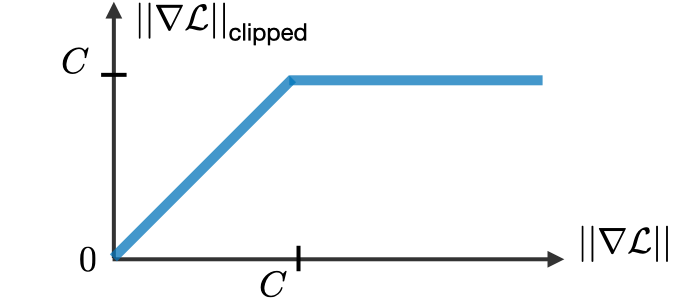
\includegraphics[scale=0.35]{gradient_clipping.png}
\end{figure}
Note that in the figure above the cost function is represented as $\pazocal{L}$

\subsubsection{A note on batching}
An important consequence of the volume of data is how the model will injest it. 
There are two places whera model injests data, namely, during training and prediction. Prediction is fairly simple, we feed the model a sufficiently large amound of data as a seed and it's predicted output will then be recursively re ingested, replacing the seed.\\
However training is more complex as there are two philosophies for ingesting data, in batches or one shot. I will briefly cover why in this paper using one shot input is neecessary. The general idea is that batches would be on the order of $10^4$ data points however with a sample rate of $22050 Hz$ this equates to around a second. Generally, music has few recognisable patterns on such time scales which is evident in the figure bellow. Due to this training must take place on larger time scales, to better recognise long term periodicity and pattern in the music. That is to say, local data patterns are unimportant to us, we only care about global, macroscopic behavior.\\
An additional factor to consider is that when batching input data is how to divide the batches. If a batch were chosen of arbitraty length, musical notes would be split in half between batches, cuaing the model to learn behavior that in not representative in music. 


We can see this behavior in an LSTM example that is heavily trained on batch data. The predicted ooutput file with the first second of a song as it's input seed is in essence just noize as in a local view that is what the model is trained on. In the figure bellow we can see clearly in the spectogram and Envelope that there is no decernable pattern. In the Sample view we can see that samples are very erratic and show no progression over time to some frequency. 
\begin{figure}[H]
\caption{Various views showing the predicted music by an LSTM with batched training data. }
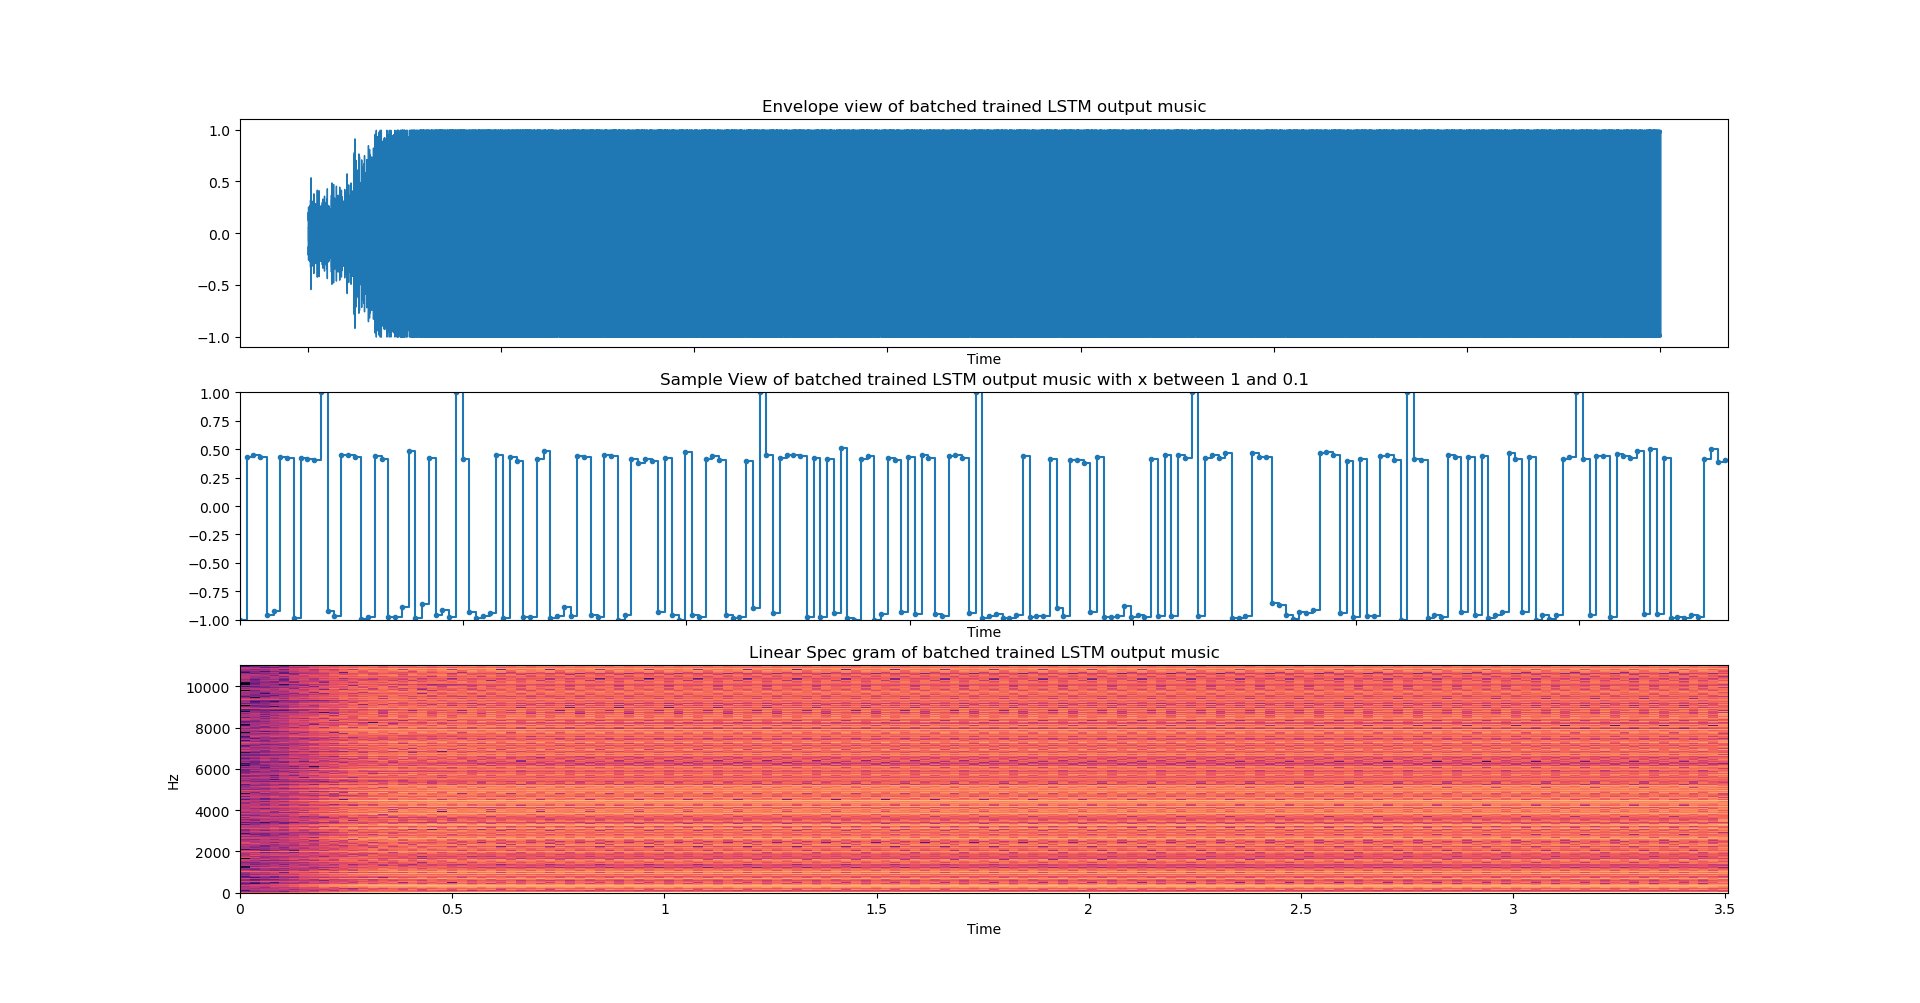
\includegraphics[scale=0.35]{batch_training.png}
\end{figure}
Due to this all training was completed in on batch in order to capture the global behavior of the song. We will see in the next section that this does, indeed, produce better results. However they are more compuatationally intesnive as each epoch one must proceed through all data points in the input data. 
\subsection{Results}
\label{sec:results}
In this section we will review various outputs of the RNN model and LSTM with various sets of hyperparameters as well analyse the qualitative and quantitave behavior of the model output. 

\subsubsection{Training and validation}
In this section we will discuss the results of training the RNN and LSTM by investigating loss progression as well as how well the model training generalises to unseen data via validation.

If we keep track of the loss at each epoch of training across several different songs while training we can produce a graph of the loss progression. For sucsessful training we expect two characteristics in this graph.
\begin{enumerate}
\item We expect to see the loss decrease consistenly over each epoch, indicating that the model is learning effectively from the input data.
\item We expect to see a rise in loss for each new song in the training dataset. However if the model is learning more general information about the music we expect each sucsessive song's increase in loss to decrease. It should be noted that this property may not be general as songs vary greatly in their similarity.
\end{enumerate}
\begin{figure}[H]
\caption{Plot of loss over 100 epochs of LSTM training on a single input song}
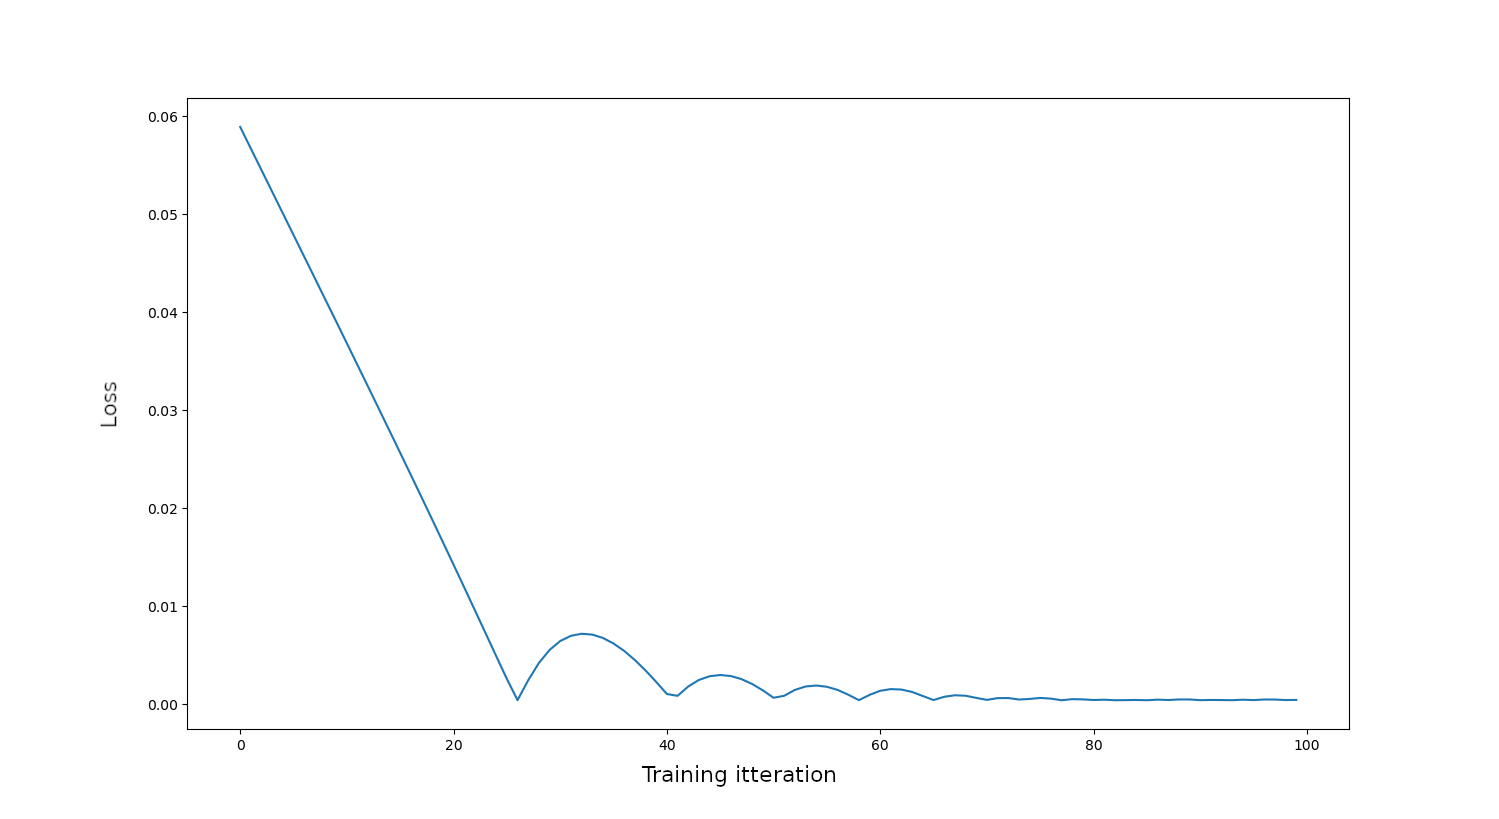
\includegraphics[scale=0.35]{loss_plot_100itr.png}
\end{figure}
Note that the loss does indeed decrease over time, however, there are two things to note. Firstly the loss has "humps" which are likely due to the optimizer attempting to find a better minimum. Secondly over time the loss settles so a near constant value, which could mean that the model is very accurate or is over fitted. If we attempt to generate a song using this model we can confirm that, indeed the model is over fitted. This can be seen in the figure bellow where the prediction is some constant value. 
\begin{figure}[H]
\caption{Prediction of 1000 amplitude samples with a classical song as the seed}
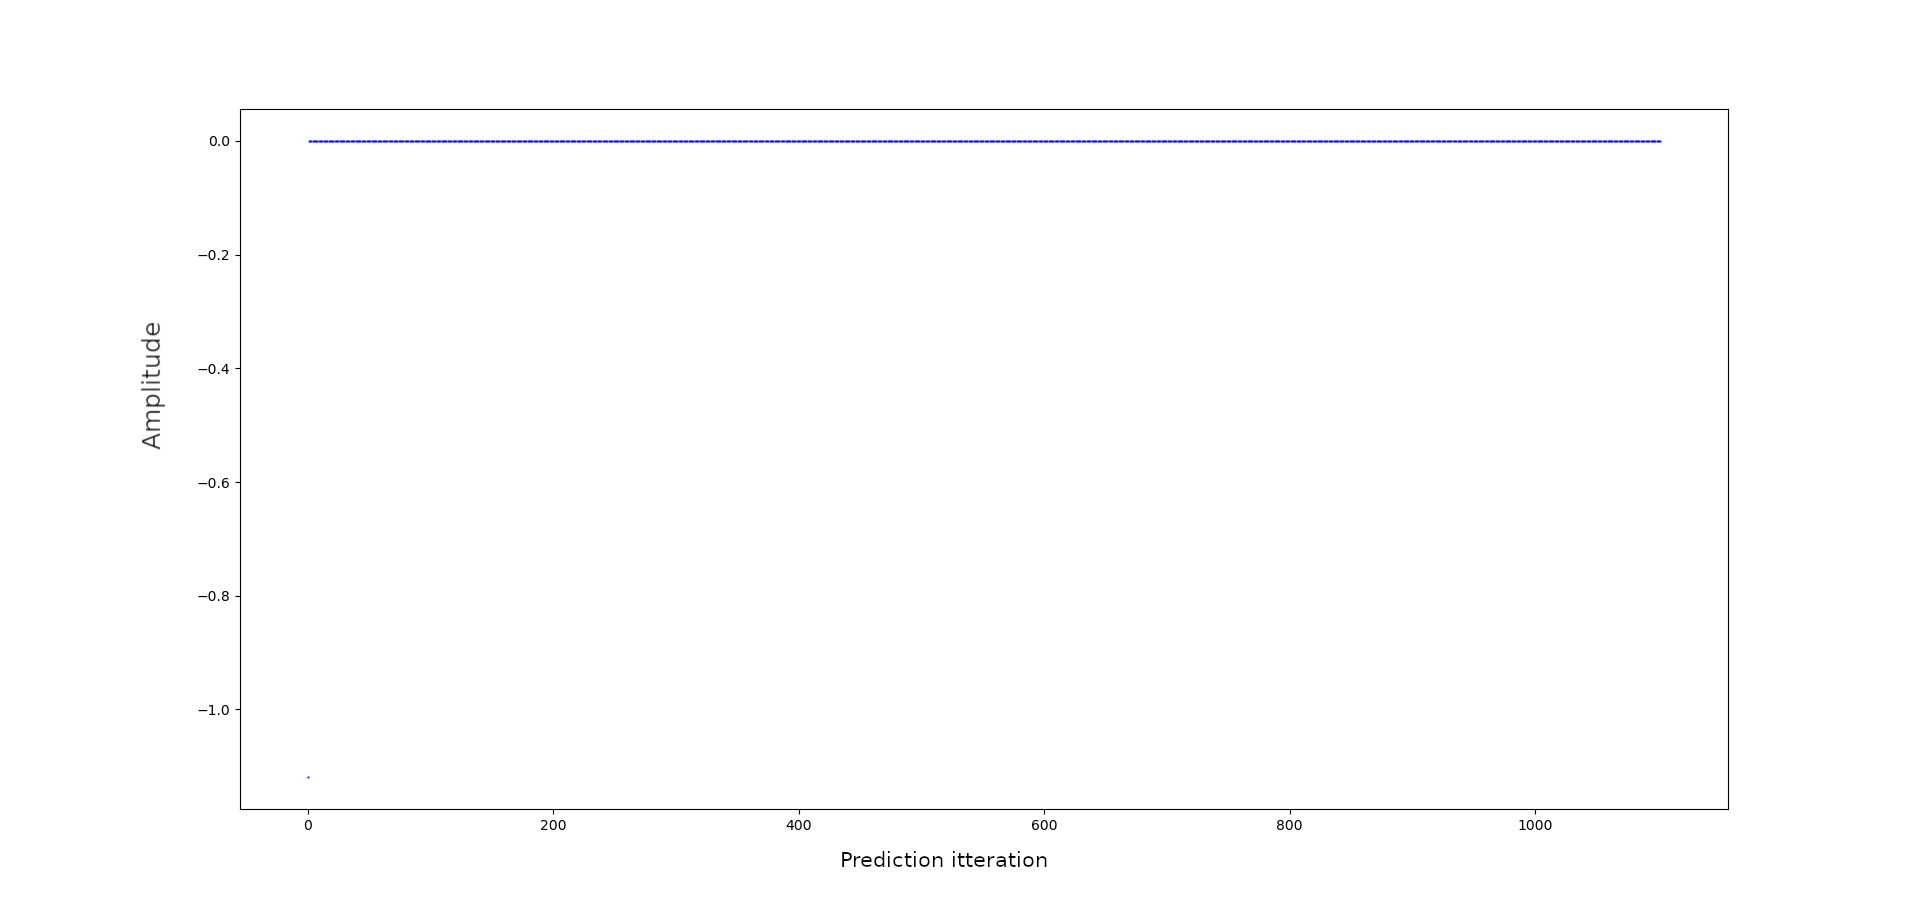
\includegraphics[scale=0.35]{overfit_1.png}
\end{figure}
Overfitting as a problem that effects most machine learning models. There are many proposed schemes to combat overfitting, a common one that we will use in this work is dropout. Dropout randomly selectes arbitrary values to completely drop. In the context of RNN's we introduce a Dropout layer on the outputs of each RNN layer and randomly select values to drop. After including a dropout scheme we can see in the figure bellow that the model no longer exhibits this over fitting behavior.
\begin{figure}[H]
\caption{Plot of loss over 100 epochs of LSTM training on a single input song}
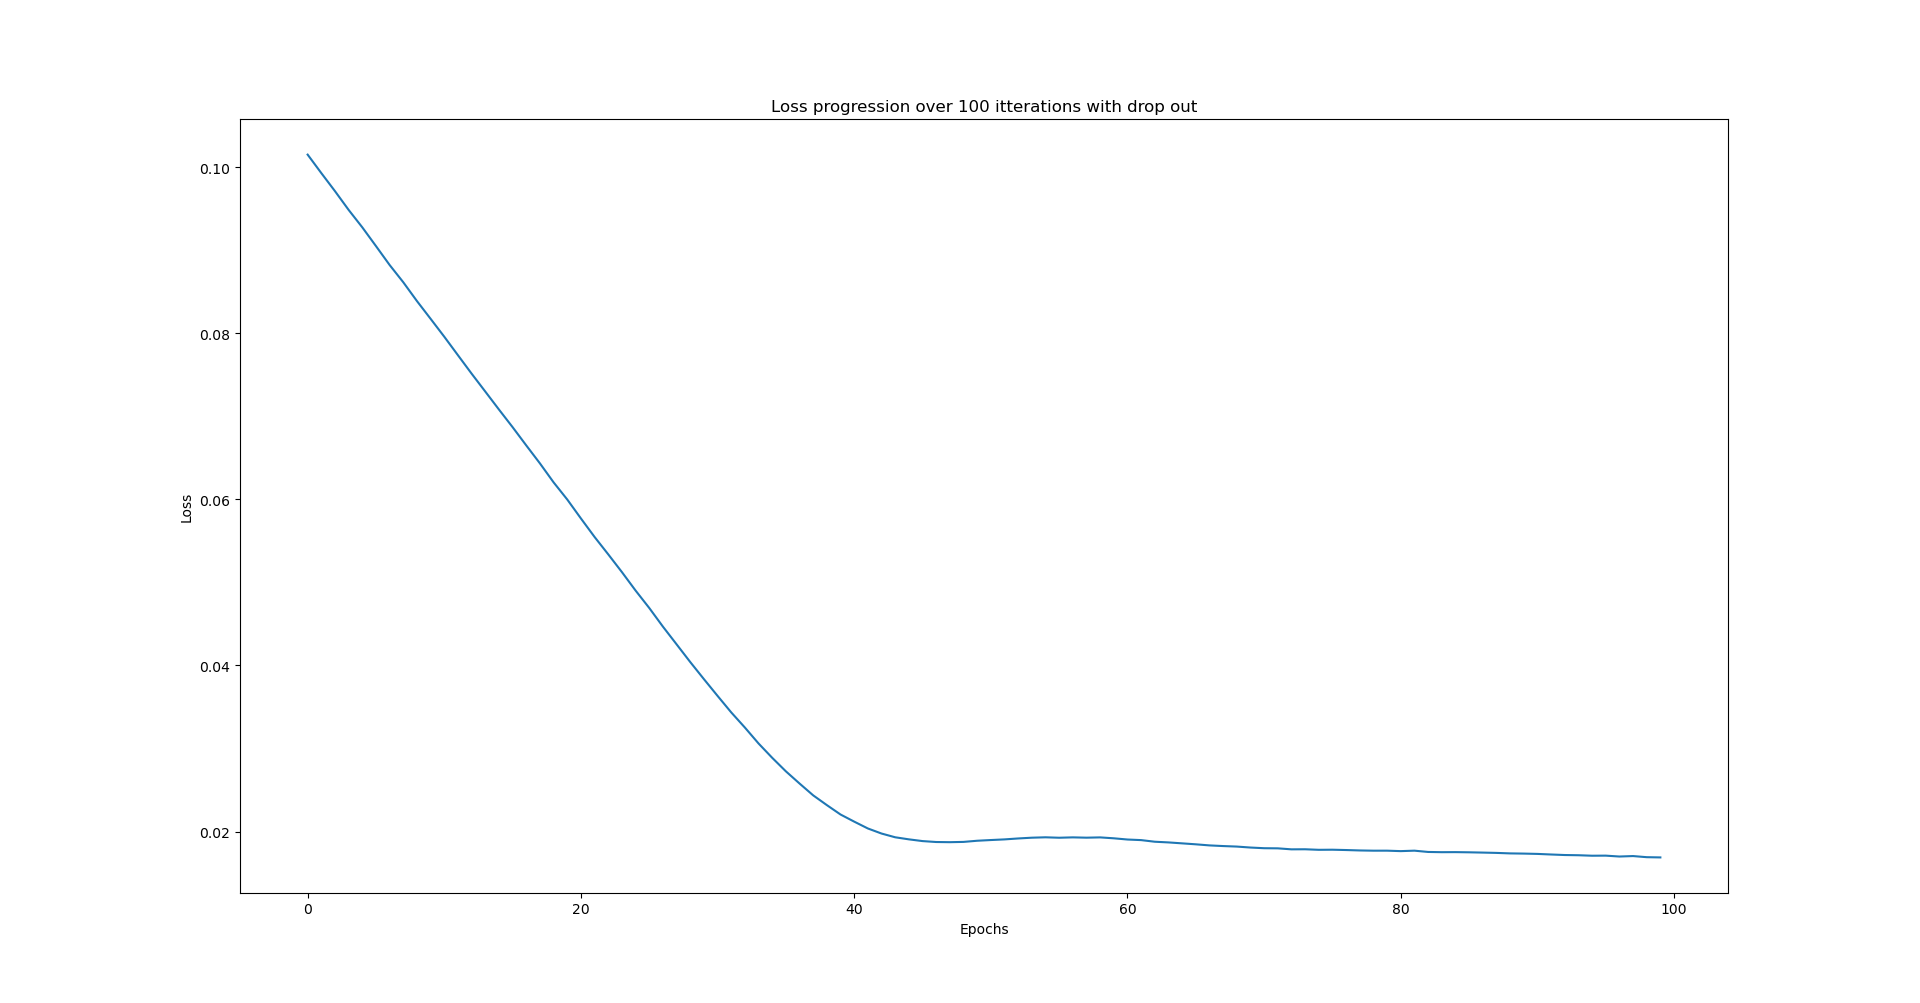
\includegraphics[scale=0.35]{loss_dropout_100itr.png}
\end{figure}
We can now verify that the model is learning generalisable knowledge. First let us plot the loss progression for training over multiple songs.
\begin{figure}[H]
\caption{Plot of loss over 100 epochs with 10 songs of 100 epochs each for LSTM}
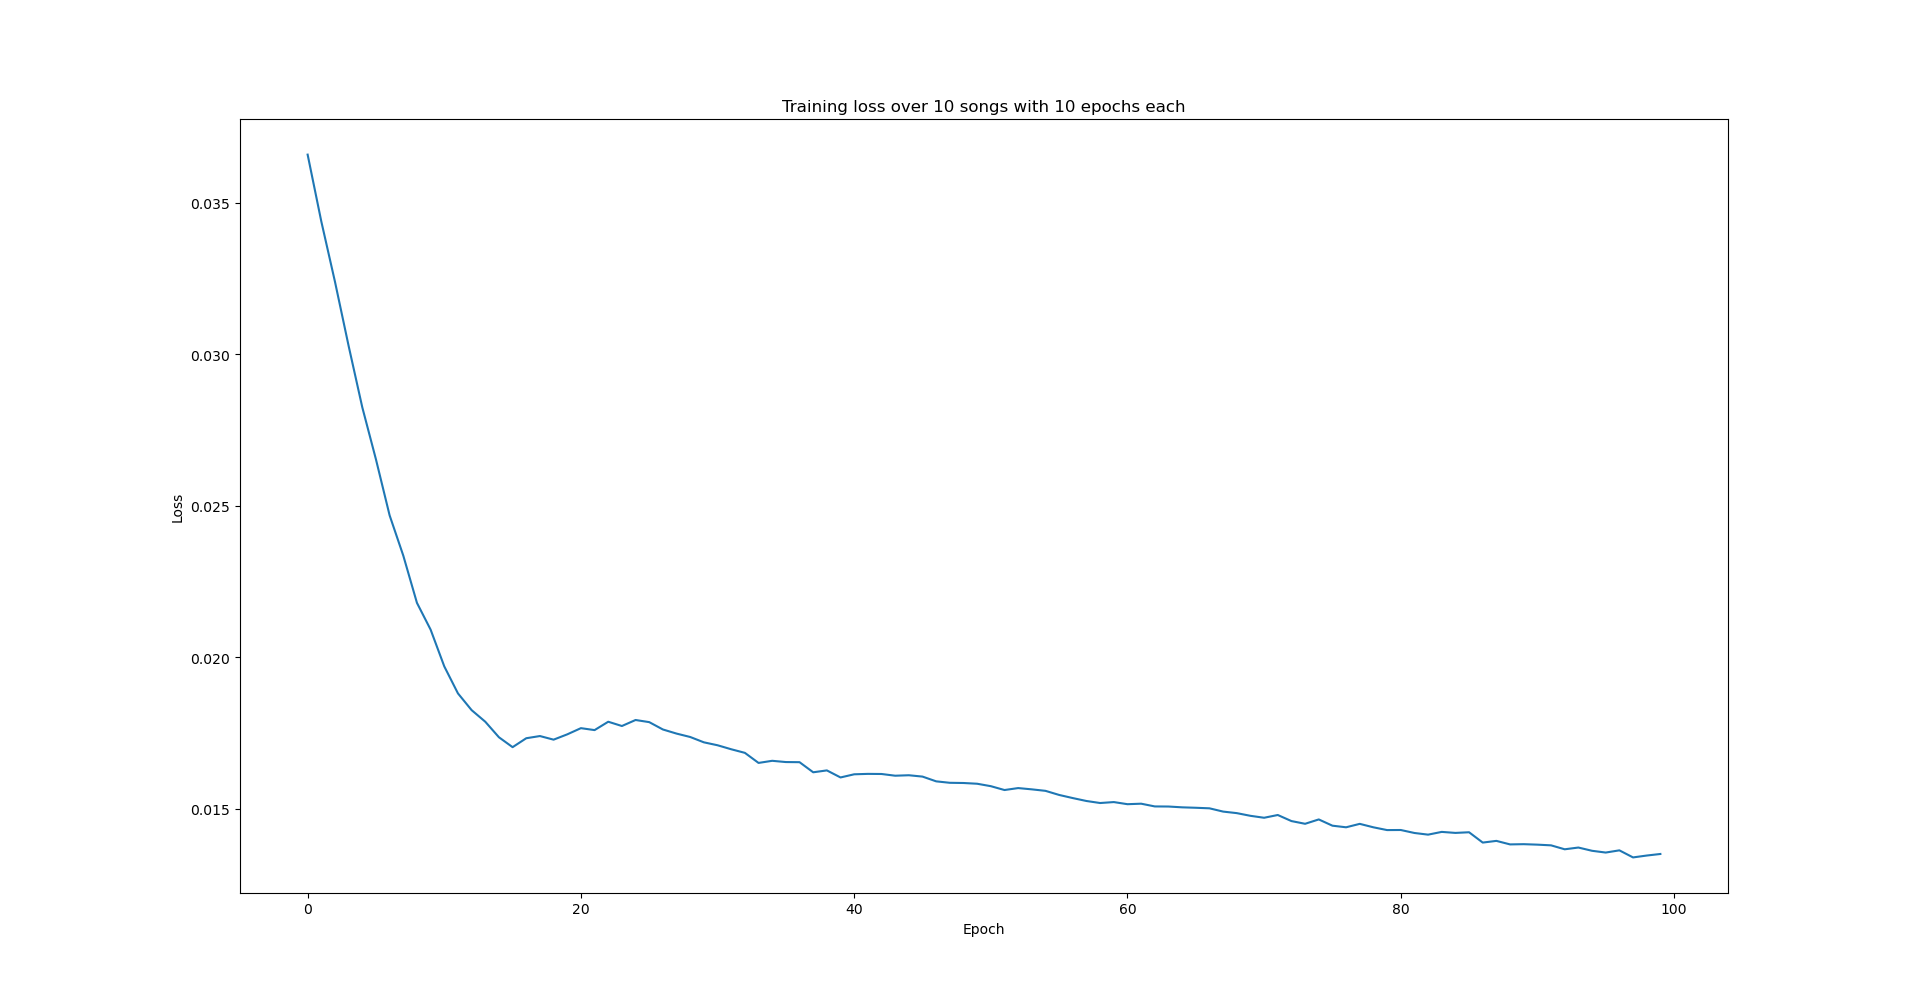
\includegraphics[scale=0.35]{loss_plot_10songs.png}
\end{figure}
After we have confirmend that the loss is decreasing as expected we need to ensure that the training is generalising to unseen data and confirm that we are not over fitting the model. To check both of these we can use a validation step during training, where periodically we give the model some unseen data as input and check the error of the prediction to the unseen data. Bellow we can see a figure showing that as the loss decreases so does the validation loss. If the model was overfit the validation loss should increase as training continues.
\begin{figure}[H]
\caption{Plot of loss over 100 epochs with 10 songs of 100 epochs each for LSTM}
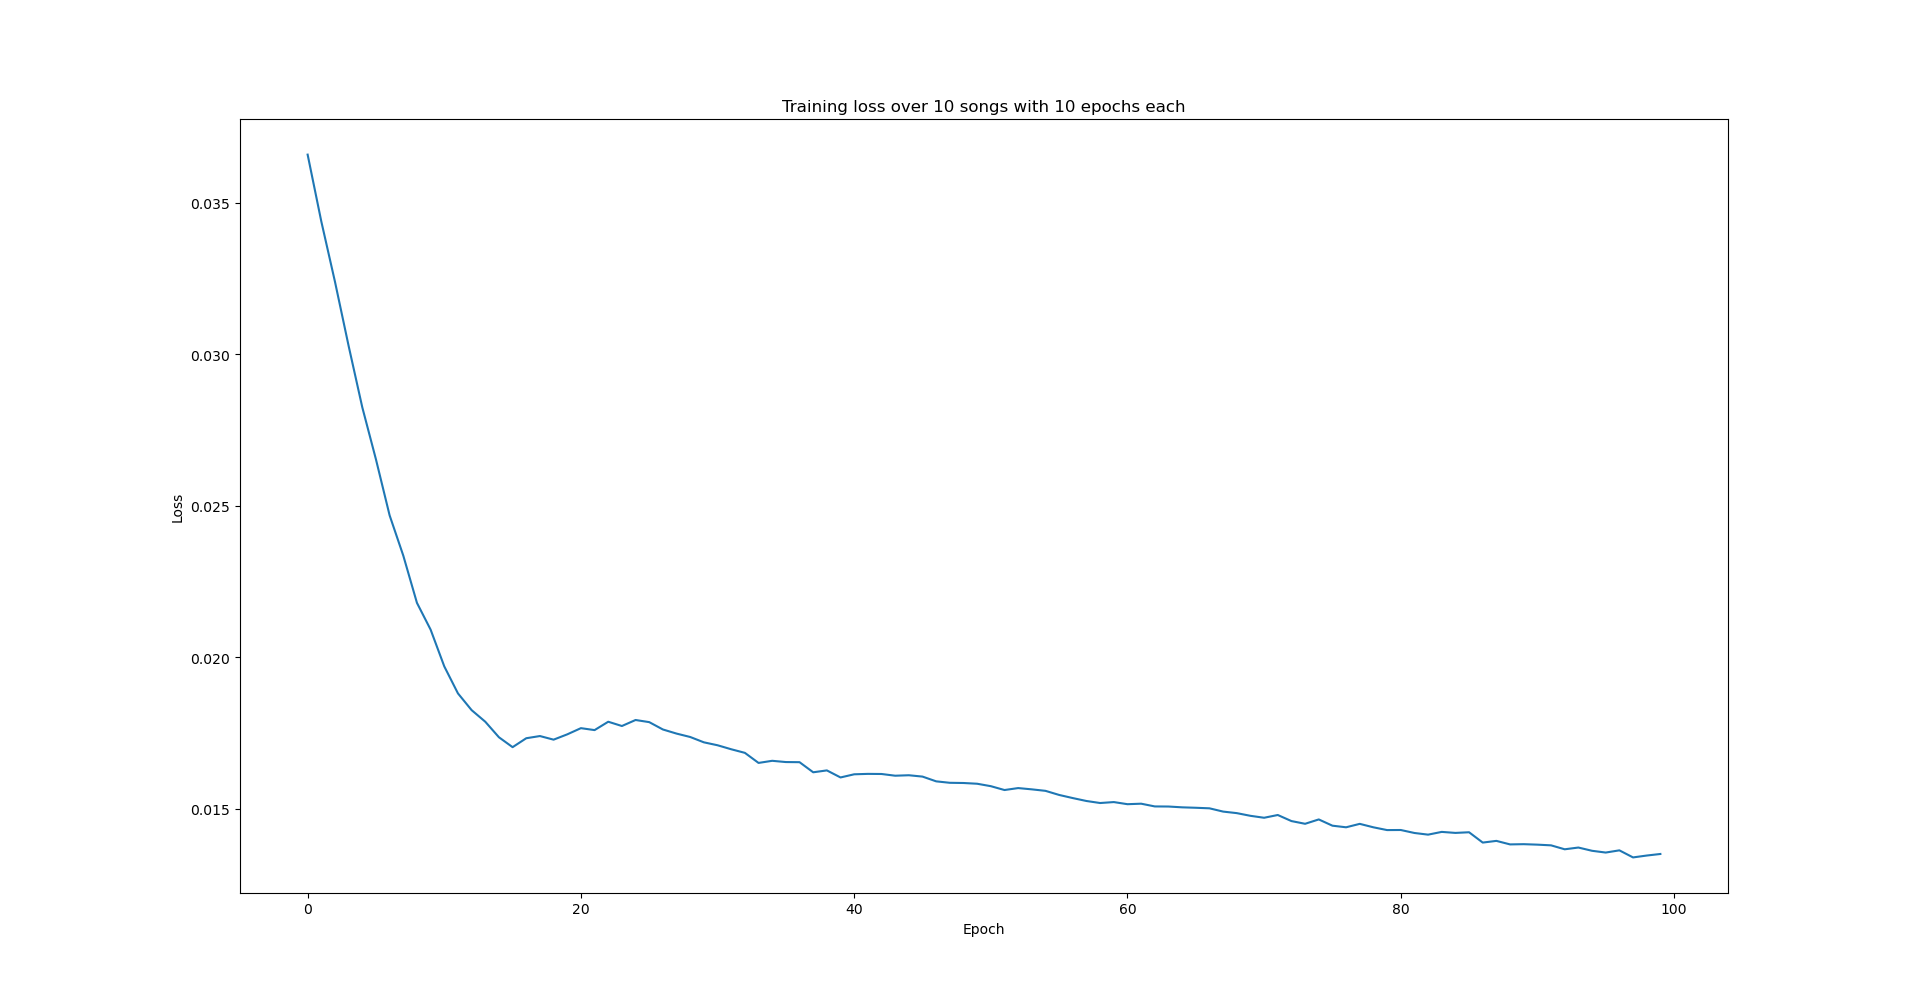
\includegraphics[scale=0.35]{loss_plot_10songs.png}
\end{figure}
\subsubsection{Initial investigation}
Before we begin to ask our model to generate completely new music it is insightful to see if the network can reproduce music. If we train the model on raw muisic samples and proceed to feed it a music it has not been trained on as input we find the following output.
\begin{figure}[H]
\caption{Showing the reproduction of an unseen song by LSTM}
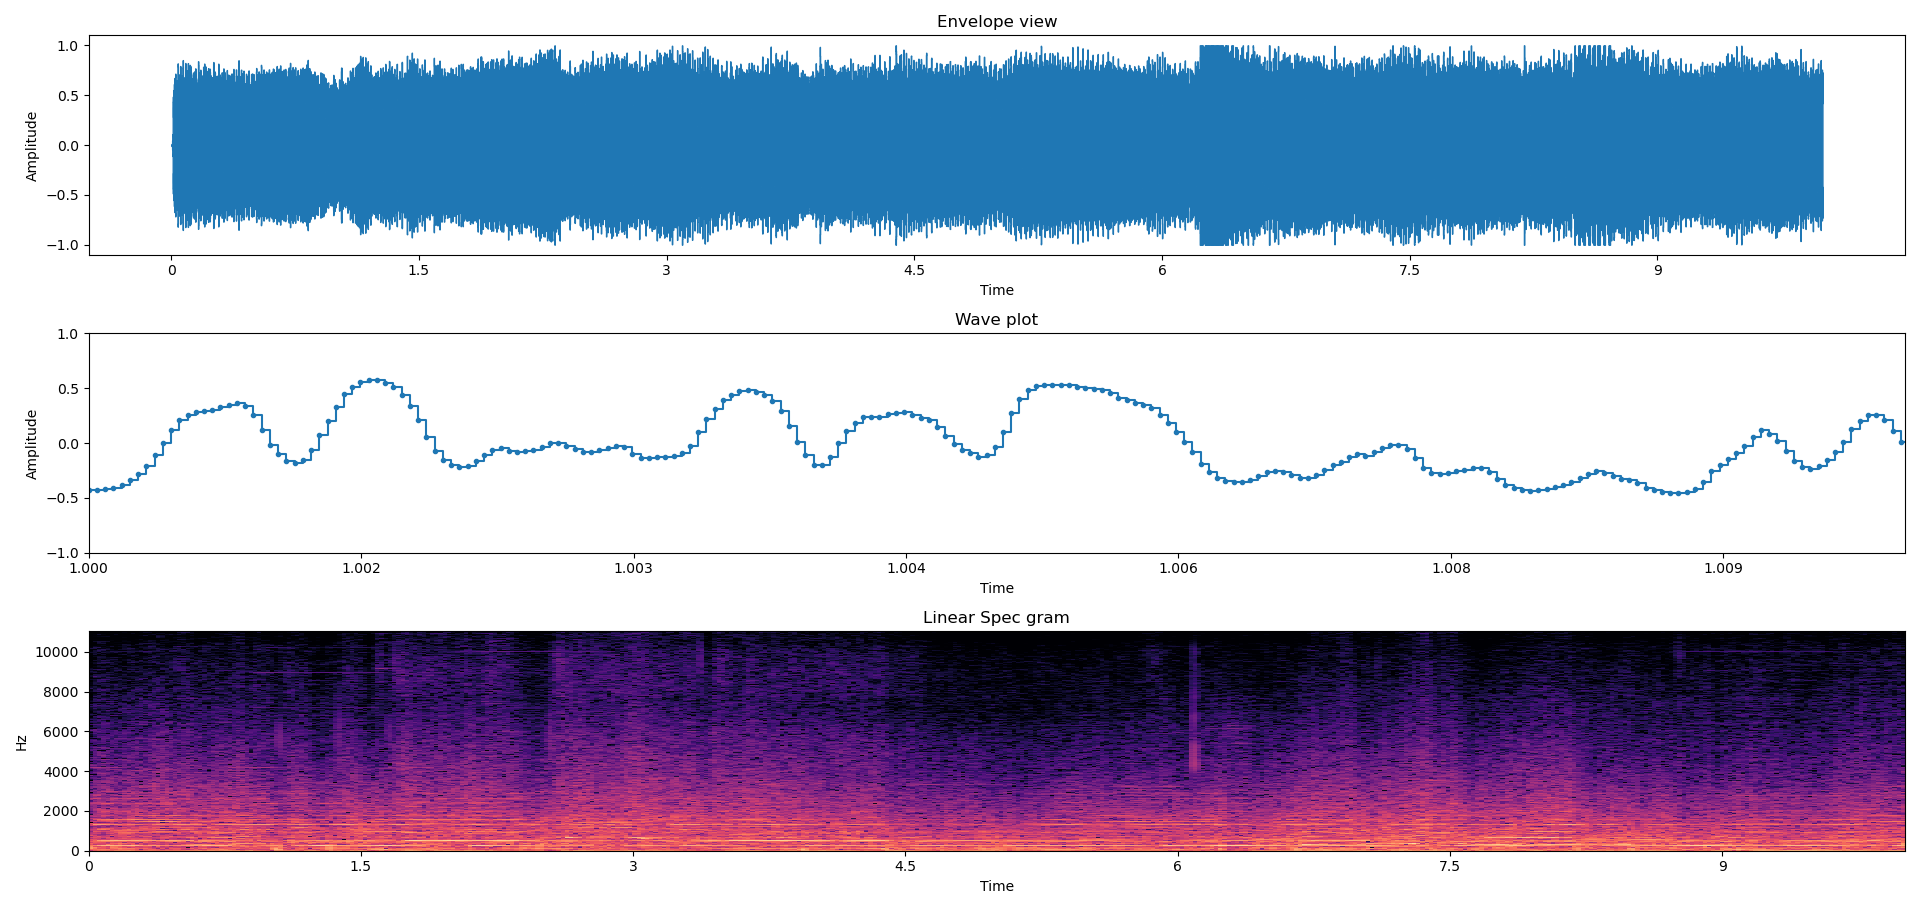
\includegraphics[scale=0.35]{reproduce1.png}
\end{figure}
We can see in the wave plot that the output is relatively smooth on small time scales with few irratic jumps. However there is still some noise in the output music which can be seen by the ill defined envelope and spectrogram. 
\begin{figure}[H]
\caption{Showing the reproduction seed of an unseen song by LSTM}
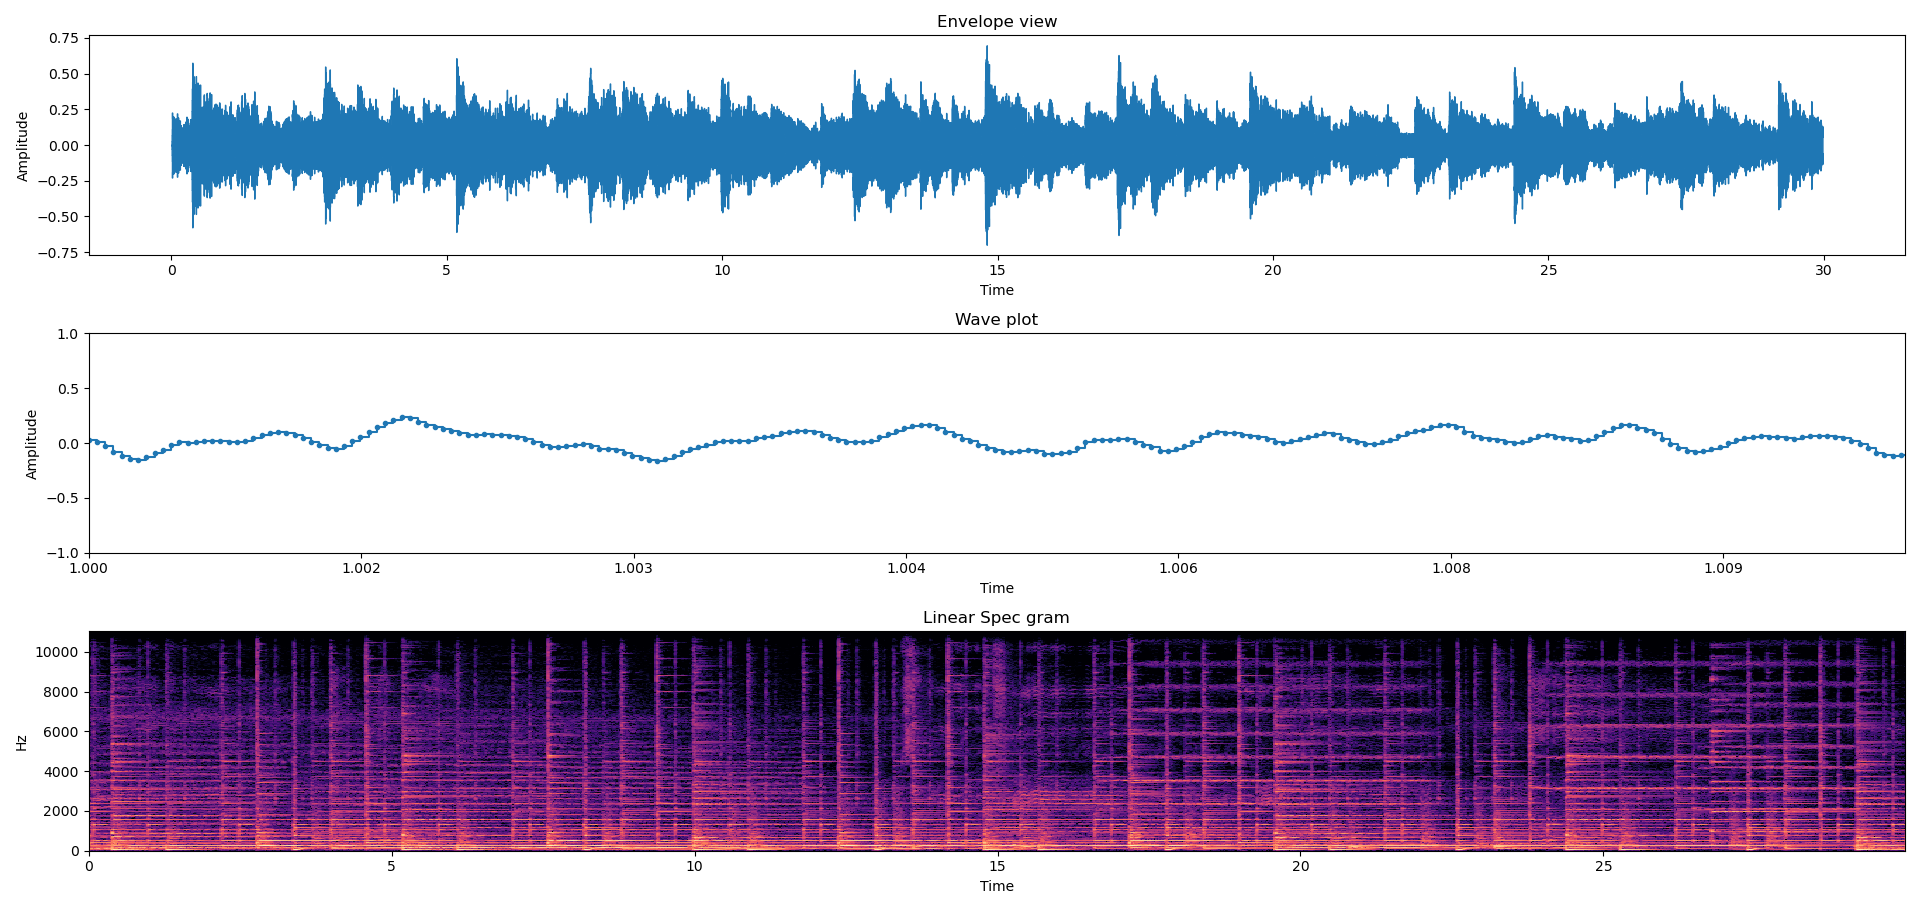
\includegraphics[scale=0.35]{reproductionSeed.png}
\end{figure}
It should be noted that although the reproduction is noisy, to the ear the music is definitely recognisable and qualitatively not unplesant. 
\subsubsection{RNN and LSTM comparison}
Here we will compare the performance of an RNN and LSTM model with the same hyperparameters where applicable. 
For a reproduction the RNN performs slightly worse than the LSTM with the same hyperparameters. The envelope and spectrogram in the figure bellow shows that the RNN reproduction contains more noise than the LSTM. Additionally, the wave plot shows that the RNN produces more erratic output that leads to a qualitatively poor listening experience. It should be noted, however, that the reproduction is still recognisable. 
\begin{figure}[H]
\caption{Showing the reproduction seed of an unseen song by RNN}
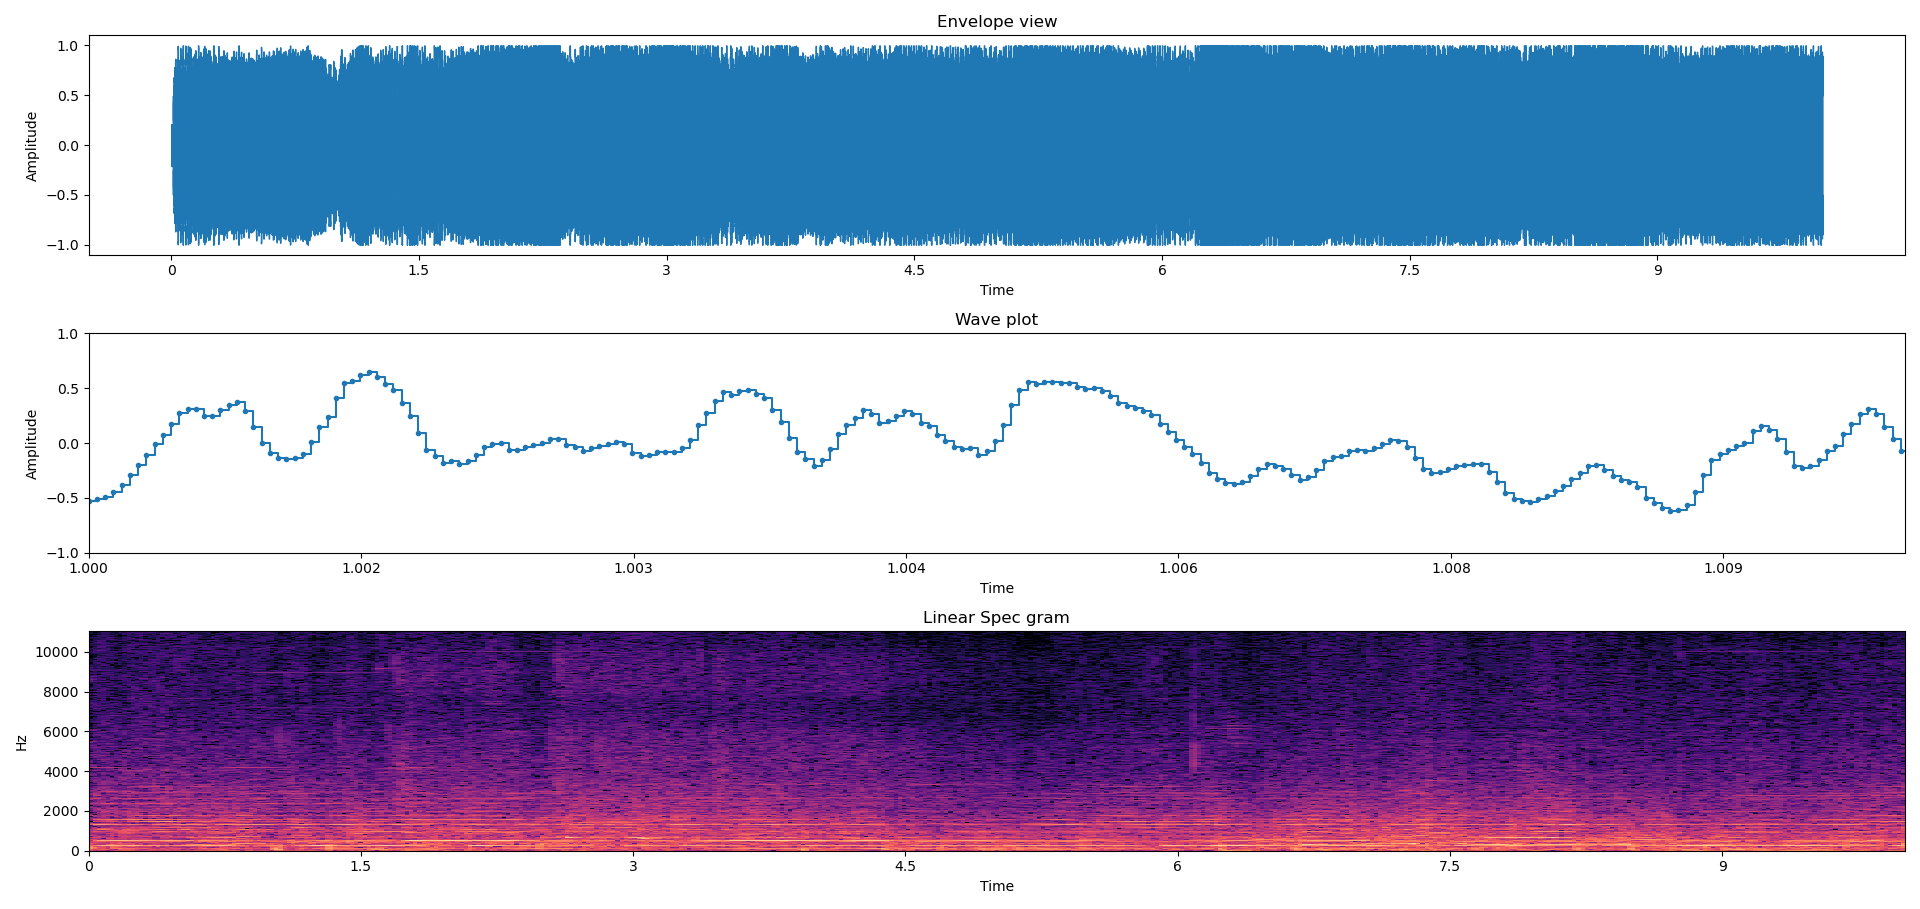
\includegraphics[scale=0.35]{RNN_Reproduction.png}
\end{figure}
The parameters are listed in the table bellow\\
\begin{tabularx}{0.8\textwidth} { 
  | >{\raggedright\arraybackslash}X 
  | >{\centering\arraybackslash}X 
  | >{\raggedleft\arraybackslash}X | }
 \hline
 Hyper-parameter & Value\\
 \hline
 Hidden Layer Dimension  & 50   \\
\hline
 RNN/LSTM Layers  & 1 \\
\hline
 Loss criterion  & MSE Loss  \\
\hline
 Optimizer  & Adam Optimizer  \\
\hline
 Learning rate  & 0.01  \\
\hline
 Genre  & Instrumental \\
\hline
 Number of songs to train on  & 5  \\
\hline
 Duration of song to train on on  & 15s \\
\hline
Gradient Clipping value & 1 \\
\hline
Dropout probability & 0.5 \\
\hline
\end{tabularx}
After approximately 5 itterations of prediction both the RNN and LSTM converge to a single output value. After reasurching this problem thoroughly there appears to be no formal works discussing the topic, however, there has been some informal discussion which often leads to the following hypotheses.
\begin{enumerate}
\item Poor scaling of data
\item Poor long term memory
\item Poor quality input data
\item Insufficient model training
\item Insufficient hyper parameter optimization
\item Insufficient model complexity
\item Insufficient data type accuracy
\item Insufficient training data
\end{enumerate}
\subsection{Adressing prediction convergence}
In this section we will layout the different model and data tuning that was used to solve the prediction value convergence problem. In the table bellow I have layed of the change and the result of such a change. 
\begin{tabularx}{0.8\textwidth} { 
  | >{\raggedright\arraybackslash}X 
  | >{\centering\arraybackslash}X 
  | >{\raggedleft\arraybackslash}X | }
 \hline
 Change & Values attempted & Result \\
 \hline
 Increasing the hidden layer dimension to address model complexity  & 10,50,256,512,1024 & Across all the values there was no change. 1024 was the limit of model size as we hit GPU memory limits   \\
\hline
 LSTM layers  & 1,2,10 & Prediction converges for all attempted values \\
\hline
 Loss criterion  & MSE Loss, MAE & Prediction converges for all attempted values  \\
\hline
 Optimizer  & Adam Optimizer, Stochastic gradient descent, ADADELTA (An Adaptive Learning Rate Method) &  Prediction converges for all attempted values \\
\hline
 Learning rate  & 1, 0.1, 0.001, 0.0001, 0.00001 & Prediction converges for all attempted values \\
\hline
 Number of songs to train on  & 1,5,100 & Prediction converges for all attempted values  \\
\hline
 Duration of song to train on on  & 0.1, 1, 5, 10, 15 & Value converges more slowly for longer durations \\
\hline
Gradient Clipping value & 0.001, 0.1, 1, 5 & Prediction converges for all attempted values\\
\hline
Dropout probability & 0.5, 0.2 & Prediction converges for all attempted values \\
\hline
Data scaling method & min-max scaling, Z-score  & Prediction converges for all attempted values \\
\hline
Training Sequence length & 2205, 11025, 22050, 110250, 100 000  & Prediction converges for all attempted values \\
\hline
Step size& 2205, 11025, 22050, 110250, 100 000  & Prediction converges for all attempted values \\
\hline
Prediction seed length & 100, 1000, 22050, 100 000  & Prediction converges for all attempted values \\
\hline
Training epochs & 1, 10, 100, 500, 1000  & Prediction converges for all attempted values \\
\hline
\end{tabularx}
The only parameter with any noticable effect is the duration of the input song. This indicates that the issue is not a hyperparameter one but rather a long term memorry issue where the LSTM struggles to maintain stable predictions past approximately 1\% of the training length which can be seen in the figure bellow where the input training duration was 1 second (22050 smaple points).  
\begin{figure}[H]
\caption{Showing the best prediction amplitude samples}
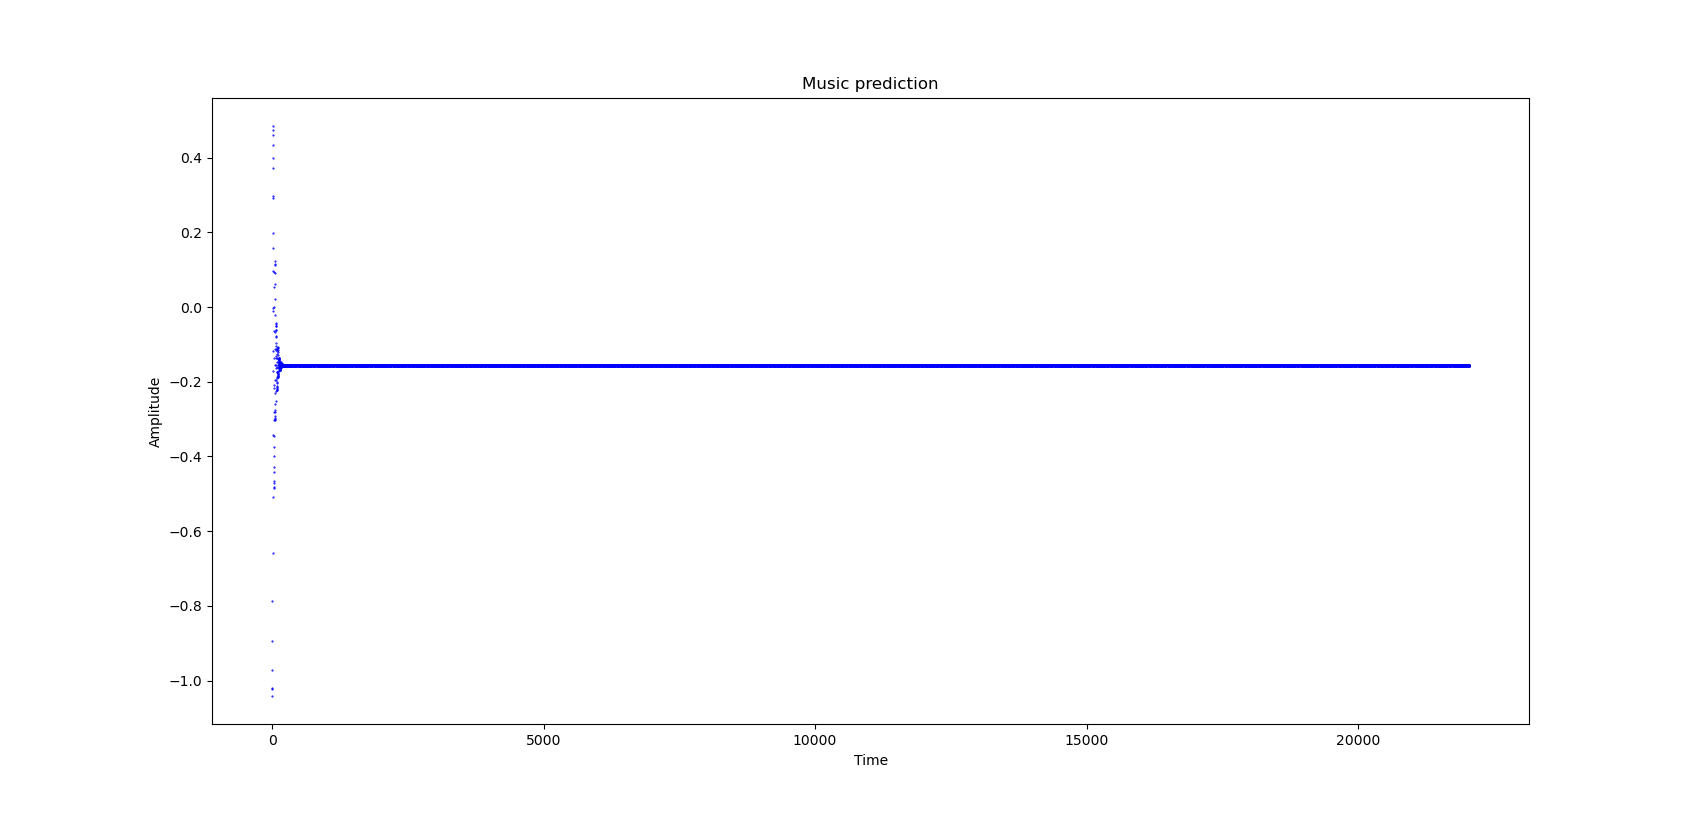
\includegraphics[scale=0.35]{better_convergence.png}
\end{figure}
This is promising as it indicates that music generation is plausible given enough computing power for sufficient training. However in this paper we have limited resources. 
\subsection{Introducing artificial noise}
A possible to the convergence of prediction values is to periodically introduce some noise to the prediction process to prevent the model from converging to a stationary value. If we notice a sequence of predictions is too similar we can inject some noise by modifying the prediction seed value at each iteration. 

\subsubsection{Fourier Transform results}
A possible cause of the convergence to a constant predicted value is that the problem is ill phrased. Moreover the problem is too nonlinear for the size of model to converge on a stable solution that doesn't converge to a single value. We can rephrase our problem from what is the next amplitude of sound that comes next to what is the next frequency that comes next. This transformation is naturally done by a Fourier Transform of the data. THe procedure is as follows use FFT to move to the frequency domain, then scale the data. Train the network on this data. Predict using a starting seed that has been transformed and scaled, then invert the scale and use an ifft sheme to obtain amplitude falues that we can write to a sound file. 

\subsection{Conclusion}
\label{sec:conclusion}

\section{References}
\printbibliography
\end{document}